\documentclass[handout]{beamer}\usepackage[]{graphicx}\usepackage[]{color}
%% maxwidth is the original width if it is less than linewidth
%% otherwise use linewidth (to make sure the graphics do not exceed the margin)
\makeatletter
\def\maxwidth{ %
  \ifdim\Gin@nat@width>\linewidth
    \linewidth
  \else
    \Gin@nat@width
  \fi
}
\makeatother

\definecolor{fgcolor}{rgb}{0.345, 0.345, 0.345}
\newcommand{\hlnum}[1]{\textcolor[rgb]{0.686,0.059,0.569}{#1}}%
\newcommand{\hlstr}[1]{\textcolor[rgb]{0.192,0.494,0.8}{#1}}%
\newcommand{\hlcom}[1]{\textcolor[rgb]{0.678,0.584,0.686}{\textit{#1}}}%
\newcommand{\hlopt}[1]{\textcolor[rgb]{0,0,0}{#1}}%
\newcommand{\hlstd}[1]{\textcolor[rgb]{0.345,0.345,0.345}{#1}}%
\newcommand{\hlkwa}[1]{\textcolor[rgb]{0.161,0.373,0.58}{\textbf{#1}}}%
\newcommand{\hlkwb}[1]{\textcolor[rgb]{0.69,0.353,0.396}{#1}}%
\newcommand{\hlkwc}[1]{\textcolor[rgb]{0.333,0.667,0.333}{#1}}%
\newcommand{\hlkwd}[1]{\textcolor[rgb]{0.737,0.353,0.396}{\textbf{#1}}}%
\let\hlipl\hlkwb

\usepackage{framed}
\makeatletter
\newenvironment{kframe}{%
 \def\at@end@of@kframe{}%
 \ifinner\ifhmode%
  \def\at@end@of@kframe{\end{minipage}}%
  \begin{minipage}{\columnwidth}%
 \fi\fi%
 \def\FrameCommand##1{\hskip\@totalleftmargin \hskip-\fboxsep
 \colorbox{shadecolor}{##1}\hskip-\fboxsep
     % There is no \\@totalrightmargin, so:
     \hskip-\linewidth \hskip-\@totalleftmargin \hskip\columnwidth}%
 \MakeFramed {\advance\hsize-\width
   \@totalleftmargin\z@ \linewidth\hsize
   \@setminipage}}%
 {\par\unskip\endMakeFramed%
 \at@end@of@kframe}
\makeatother

\definecolor{shadecolor}{rgb}{.97, .97, .97}
\definecolor{messagecolor}{rgb}{0, 0, 0}
\definecolor{warningcolor}{rgb}{1, 0, 1}
\definecolor{errorcolor}{rgb}{1, 0, 0}
\newenvironment{knitrout}{}{} % an empty environment to be redefined in TeX

\usepackage{alltt}

\usepackage{default}
\usepackage{animate} %need the animate.sty file 
\usepackage{graphicx}
%\graphicspath{{/home/sahir/Dropbox/jobs/laval/minicours/slides/}}
\usepackage{hyperref, url}
%\usepackage[round,sort]{natbib}   % bibliography omit 'round' option if you prefer square brackets
%\bibliographystyle{apalike}
\usepackage{biblatex}
\bibliography{bib.bib}
% Removes icon in bibliography
\setbeamertemplate{bibliography item}[text]

\usepackage[normalem]{ulem}

\setbeamertemplate{theorems}[numbered]



%\newtheorem{prop}{Proposition}
%\newenvironment{theoremc}[1]
%{\begin{shaded}\begin{theorem}[#1]}
%		{\end{theorem}\end{shaded}}
	
%\newtheorem{examplefirst}{Example}
%\newtheorem{examplesecond}{Example}
%\newenvironment<>{examplefirst}[1][]{%
%	\setbeamercolor{block title example}{bg=lightgray}%
%	\begin{example}#2[#1]}{\end{example}}
%\newenvironment<>{examplesecond}[1][]{%
%	\setbeamercolor{block title example}{fg=white,bg=blue!75!black}%
%	\begin{example}#2[#1]}{\end{example}}	

%\usepackage{amsthm}


\usepackage[figurename=Fig.]{caption}
\usepackage{subfig}
\usepackage{tikz, pgfplots,epsfig}
\usetikzlibrary{arrows,shapes.geometric}
\usepackage{color, colortbl,xcolor}
\definecolor{lightgray}{RGB}{200,200,200}
\definecolor{palegray}{RGB}{221,221,221}
\definecolor{myblue}{RGB}{0,89,179}
\usepackage{comment}
\setbeamercolor{frametitle}{fg=myblue}
\setbeamercolor{section in head/foot}{bg=myblue, fg=white}
\setbeamercolor{author in head/foot}{bg=myblue}
\setbeamercolor{date in head/foot}{bg=myblue}

\usepackage{shadethm}
%\colorlet{shadecolor}{blue!15}
\colorlet{shadecolor}{palegray}
%\setlength{\shadeboxrule}{.4pt}

\newshadetheorem{thm}{Theorem}
\newshadetheorem{defm}{Definition}
\newshadetheorem{exm}{Exercise}
\newshadetheorem{remarkm}{Remark}
%\definecolor{shadethmcolor}{HTML}{EDF8FF}
\definecolor{shadethmcolor}{RGB}{221,221,221}
%\definecolor{shaderulecolor}{HTML}{45CFFF}
\definecolor{shaderulecolor}{RGB}{0,89,179}
\setlength{\shadeboxrule}{.4pt}


\usepackage{array}
\newcolumntype{L}{>{\centering\arraybackslash}m{3cm}} % used for text wrapping in ctable
\usepackage{ctable}
\usepackage[utf8]{inputenc}
\usepackage{fontenc}
\usepackage{pifont}% http://ctan.org/pkg/pifont
\newcommand{\cmark}{\ding{51}}%
\newcommand{\xmark}{\ding{55}}%
\def\widebar#1{\overline{#1}}
\definecolor{whitesmoke}{rgb}{0.96, 0.96, 0.96}

\usepackage{amssymb}
\usepackage{amsmath}

\usepackage{bm}
\def\transpose{{\sf{T}}}
\def\E{{\skew0\bm{E}}}
\def\Xvec{{\skew0\bm{X}}}
\def\Xveca{{\skew0\bm{X}}_1}
\def\Xvecb{{\skew0\bm{X}}_2}

\def\Yvec{{\skew0\bm{Y}}}
\def\bmY{{\skew0\bm{Y}}}
\def\bmX{{\skew0\bm{X}}}
\def\bmy{{\skew0\bm{y}}}
\def\bmG{{\skew0\bm{G}}}
\def\bmS{{\skew0\bm{S}}}
\def\bmA{{\skew0\bm{A}}}
\def\bmB{{\skew0\bm{B}}}
\def\bmD{{\skew0\bm{D}}}
\def\bmI{{\skew0\bm{I}}}
\def\bmV{{\skew0\bm{V}}}
\def\bmU{{\skew0\bm{U}}}
\def\bv{{\skew0\bm{v}}}
\def\bw{{\skew0\bm{w}}}
\def\bmm{{\skew0\bm{m}}}
\def\bmzero{{\skew0\bm{0}}}
\def\bx{{\skew0\bm{x}}}
\def\xveca{{\skew0\bm{x}}_1}
\def\xvecb{{\skew0\bm{x}}_2}

\def\N{{\skew0\mathcal{N}}}
\def\T{{\small T}}

\def\mvec{{\skew0\bm{m}}}
\def\bmmu{{\skew0\bm{\mu}}}
\def\muvec{{\skew0\bm{\mu}}}
\def\balpha{{\skew0\bm{\alpha}}}
\def\bbeta{{\skew0\bm{\beta}}}
\def\bmtheta{{\skew0\bm{\theta}}}
\def\btheta{{\skew0\bm{\theta}}}

\def\cvec{{\skew0\mathbf{c}}}

\def\Xbar{\overline{X}}

\definecolor{lightgray}{rgb}{0.91,0.91,0.91}
\definecolor{purpleblue}{rgb}{0.50,0.50,1.00}



\usepackage{fontspec}
%\setsansfont{Fira Sans}
%\setmonofont{Fira Mono}
\setsansfont[ItalicFont={Fira Sans Light Italic},BoldFont={Fira Sans},BoldItalicFont={Fira Sans Italic}]{Fira Sans Light}
\setmonofont[BoldFont={Fira Mono Medium}]{Fira Mono}


\setbeamercolor{itemize item}{fg=myblue}
\setbeamertemplate{itemize item}[square]

\setbeamertemplate{navigation symbols}{\usebeamercolor[fg]{title in head/foot}\usebeamerfont{title in head/foot}\insertframenumber}
\setbeamertemplate{footline}{}

\newtheorem{proposition}[theorem]{Proposition}
\newtheorem{exercise}[theorem]{Exercise}

\titlegraphic{\hfill
\includegraphics[height=1cm]{mcgill_logo.png}}


%% You also use hyperref, and pick colors 
\hypersetup{colorlinks,citecolor=orange,filecolor=red,linkcolor=brown,urlcolor=blue}

\newcommand {\framedgraphiccaption}[2] {
	\begin{figure}
		\centering
		\includegraphics[width=\textwidth,height=0.8\textheight,keepaspectratio]{#1}
		\caption{#2}
	\end{figure}
}

\newcommand {\framedgraphic}[1] {
	\begin{figure}
		\centering
		\includegraphics[width=\textwidth,height=0.9\textheight,keepaspectratio]{#1}
	\end{figure}
}


\AtBeginSection[]{
	\begin{frame}
		\vfill
		\centering
		\begin{beamercolorbox}[sep=8pt,center,shadow=true,rounded=true]{title}
			\usebeamerfont{title}\insertsectionhead\par%
		\end{beamercolorbox}
		\vfill
	\end{frame}
}

\newcommand\Wider[2][3em]{%
	\makebox[\linewidth][c]{%
		\begin{minipage}{\dimexpr\textwidth+#1\relax}
			\raggedright#2
		\end{minipage}%
	}%
}
\IfFileExists{upquote.sty}{\usepackage{upquote}}{}
\begin{document}
%\sffamily



%\title{Introduction to Regression Trees}
%\author{Sahir Bhatnagar \inst{1}}
%\author[shortname]{Sahir Rai Bhatnagar, PhD Candidate (Biostatistics) }
%\institute[shortinst]{Department of Epidemiology, Biostatistics and Occupational Health}

\title{Bootstrap Confidence Intervals}
\author{Sahir Bhatnagar and James Hanley}
\institute{
	EPIB 607\\
	Department of Epidemiology, Biostatistics, and Occupational Health\\
	McGill University\\
	
	\vspace{0.1 in}
	
	\texttt{sahir.bhatnagar@mcgill.ca}\\
	\texttt{\url{https://sahirbhatnagar.com/EPIB607/}}}

%\date

\maketitle

\section{Review of Confidence Intervals}

\begin{frame}{Sampling Distribution}

\begin{defm}[Sampling Distribution]
	\begin{itemize}
		\item The sampling distribution of a statistic is the distribution of values taken by the statistic in \textbf{all possible samples of the same size} from the same population.
		\item The standard deviation of a sampling distribution is called a \textbf{standard error}
	\end{itemize} 
\end{defm}


\end{frame}


\begin{frame}[fragile]{Sampling Distributions}

\begin{knitrout}\scriptsize
\definecolor{shadecolor}{rgb}{0.969, 0.969, 0.969}\color{fgcolor}\begin{figure}

{\centering 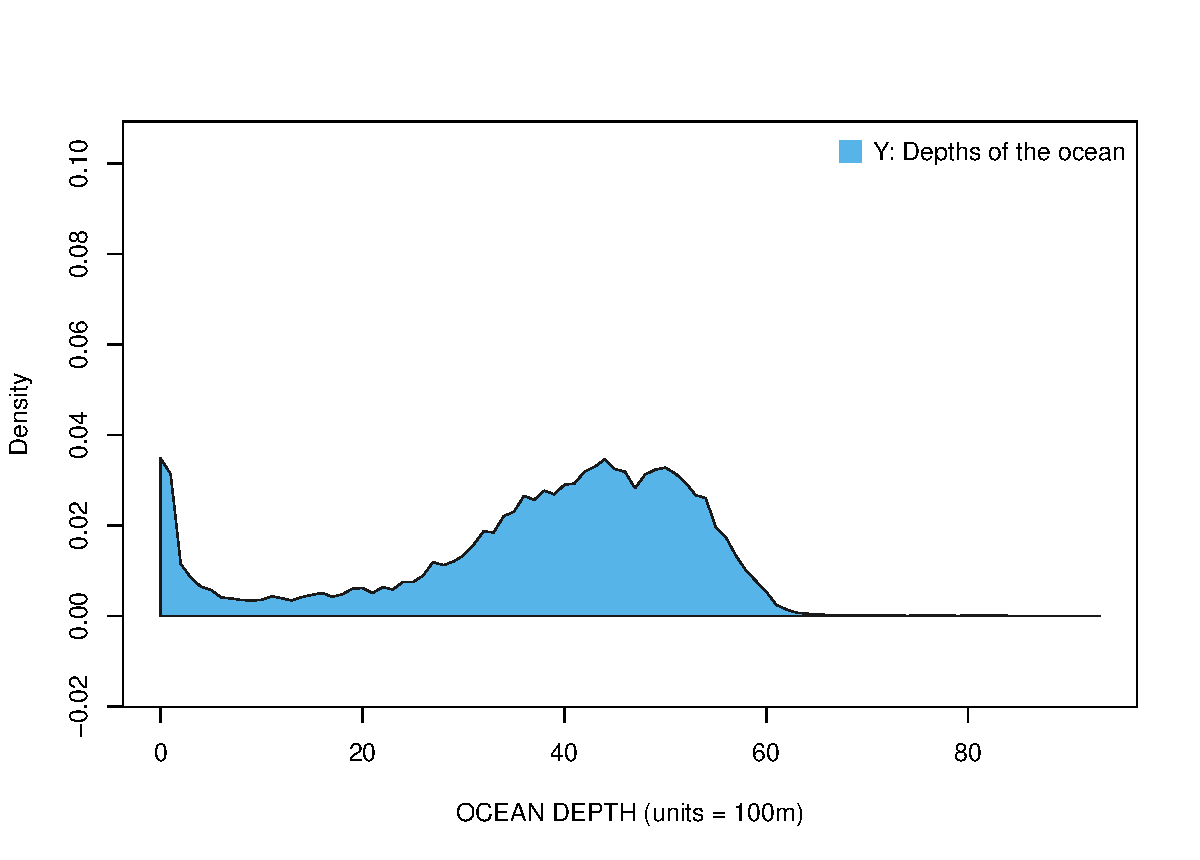
\includegraphics[width=1\linewidth]{figure/unnamed-chunk-1-1} 

}

\caption[Ideal world]{Ideal world. Sampling distributions are obtained by drawing repeated samples from the population, computing the statistic of interest for each, and collecting (an infinite number of) those statistics as the sampling distribution}\label{fig:unnamed-chunk-1}
\end{figure}


\end{knitrout}

\end{frame}



\begin{frame}{Sampling Distribution}

\Wider[4em]{
\begin{figure}
	\centering
	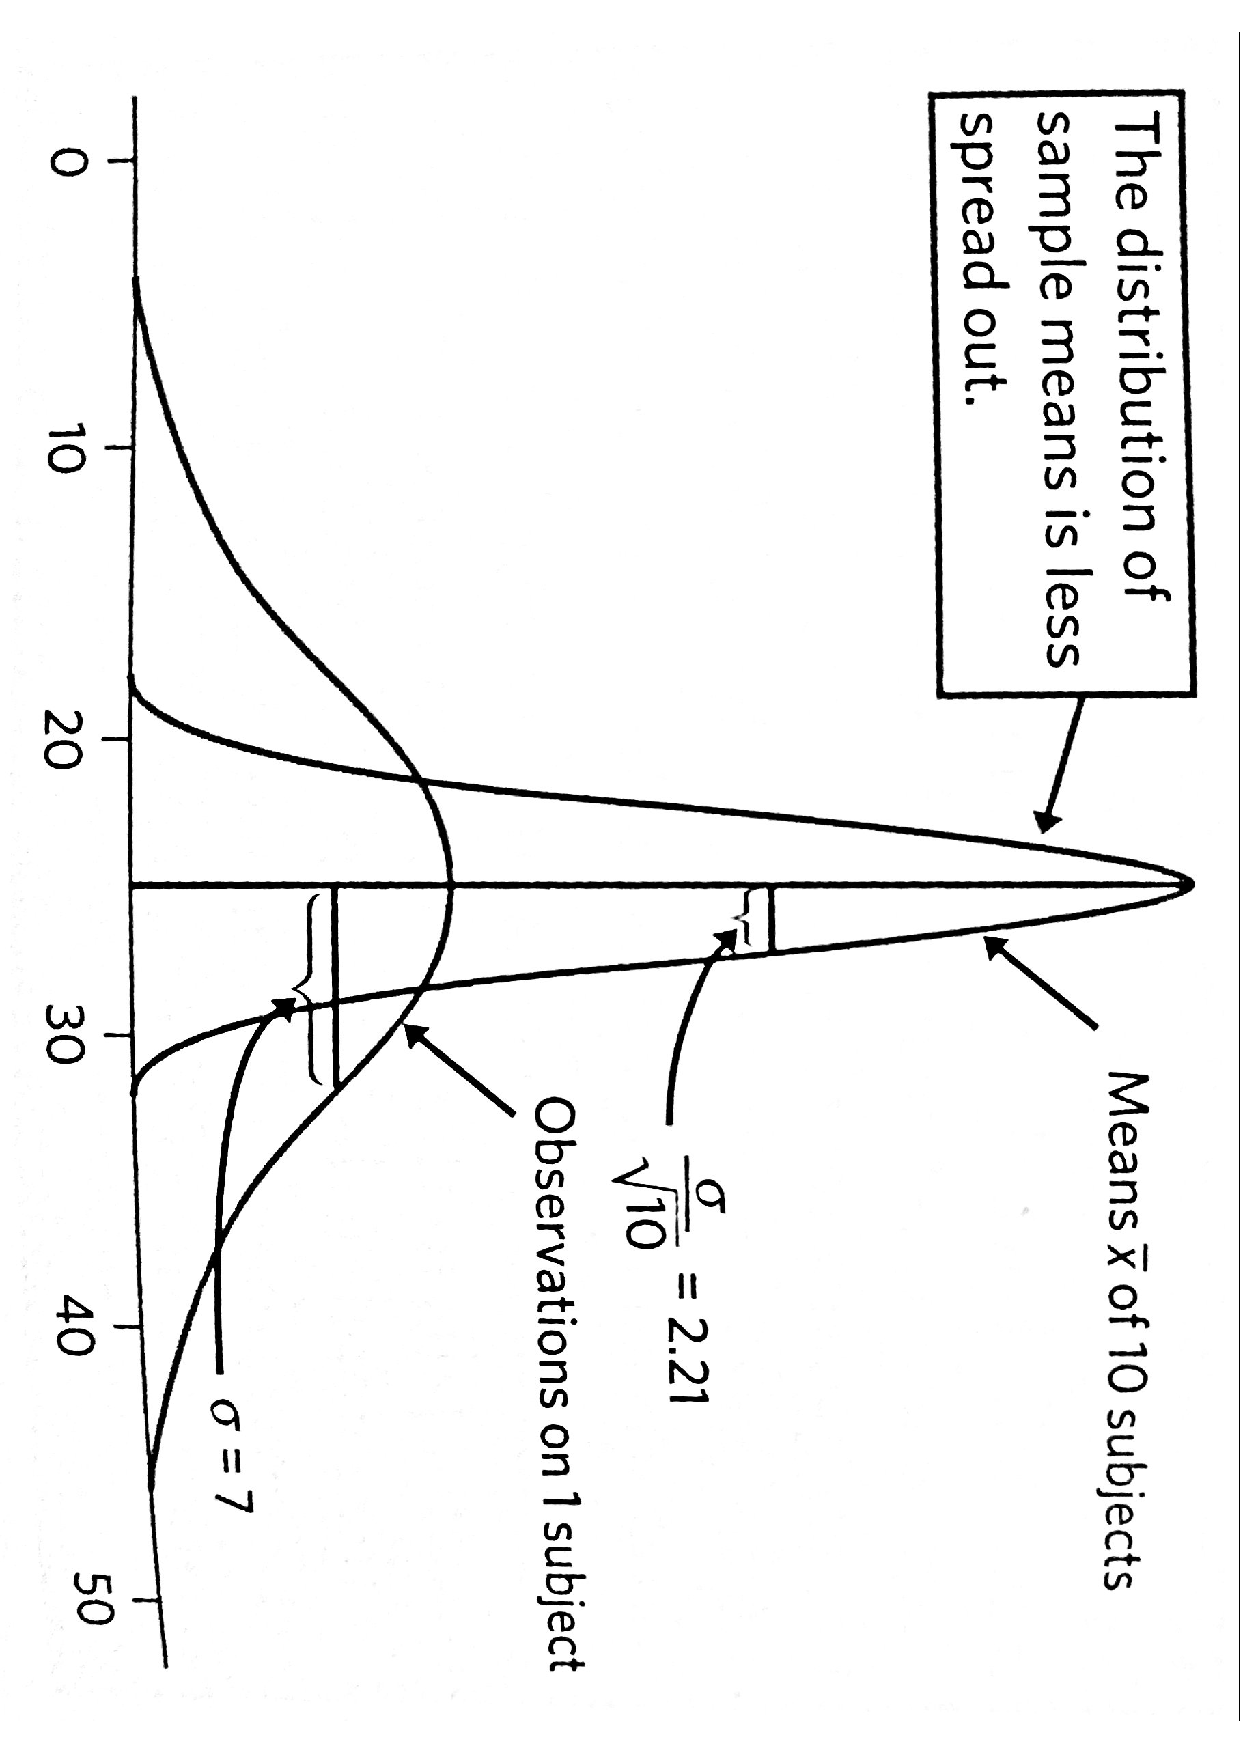
\includegraphics[scale=0.33, angle=90]{samplingdist_B_M.pdf}
	\caption{Averages are less variable than individual observations}
\end{figure}
}

\end{frame}



\frame{\frametitle{Traditional way to calculate CIs}
	How to construct a CI for the population mean?
	\begin{itemize}
		\item The \textbf{CLT} gives us that $\overline{y} \sim
		\mathcal{N}(\mu,\sigma/\sqrt{n})$ is approximately true when $n$ is
		large. \pause 
		\item We can standardize, to get $Z = \frac{\overline{y}-\mu}{\sigma/\sqrt{n}} \sim
		\mathcal{N}(0,1)$. \pause
		\item To find a CI with confidence level $\mathcal{C} = 1-\alpha$, we must calculate the critical value $z^*$  such that \begin{equation}
		P(-z^* < Z < z^*) = \mathcal{C} = 1-\alpha
		\end{equation}
		where $\alpha$ is the significance level \pause
		\begin{itemize}
			\item That is, we want the value $z^*$ that gives a
			\textit{lower tail probability} of $(1-\mathcal{C})/2 = \alpha / 2$. \pause
			\item Often this value is denoted $z^* = z_{\alpha/2}$; thus we have \[P(Z <
			-z_{\alpha/2}) = \alpha/2,\] and \[P(Z >
			z_{\alpha/2}) = \alpha/2.\]
		\end{itemize}
	\end{itemize}
} 

\begin{comment}
\frame{\frametitle{CIs for $\mu$ when $\sigma^2$ is known} Then we
	have:
	\[\begin{array}{ccl} 1-\alpha & = & P(-z_{\alpha/2} < Z < z_{\alpha/2})\\
	& & \\ & = & P\left(-z_{\alpha/2} < \frac{\overline{y}-\mu}{\sigma/\sqrt{n}} < z_{\alpha/2}\right)\\
	& & \\ & = & P\left(-z_{\alpha/2} <
	\frac{\mu-\overline{y}}{\sigma/\sqrt{n}} <
	z_{\alpha/2}\right)\\ \pause
	& & \\ & = & P\left(-z_{\alpha/2}\frac{\sigma}{\sqrt{n}} <
	\mu-\overline{y} <
	z_{\alpha/2}\frac{\sigma}{\sqrt{n}}\right)\\ \pause
	& & \\ & = & P\left(\overline{y}-z_{\alpha/2}\frac{\sigma}{\sqrt{n}}
	< \mu < \overline{y}+z_{\alpha/2}\frac{\sigma}{\sqrt{n}}\right)\\ & & \\
	\end{array}\]
	
	So a $(1-\alpha)$100\% CI for $\mu$ is
	\textcolor{blue}{$\overline{y}\pm
		z_{\alpha/2}\frac{\sigma}{\sqrt{n}}$.} }
\end{comment}

\begin{frame}{Traditional way to calculate CIs}

\Wider[2em]{
	
	
	\begin{columns}
		\begin{column}{0.5\textwidth}
			\begin{figure}
				\centering
				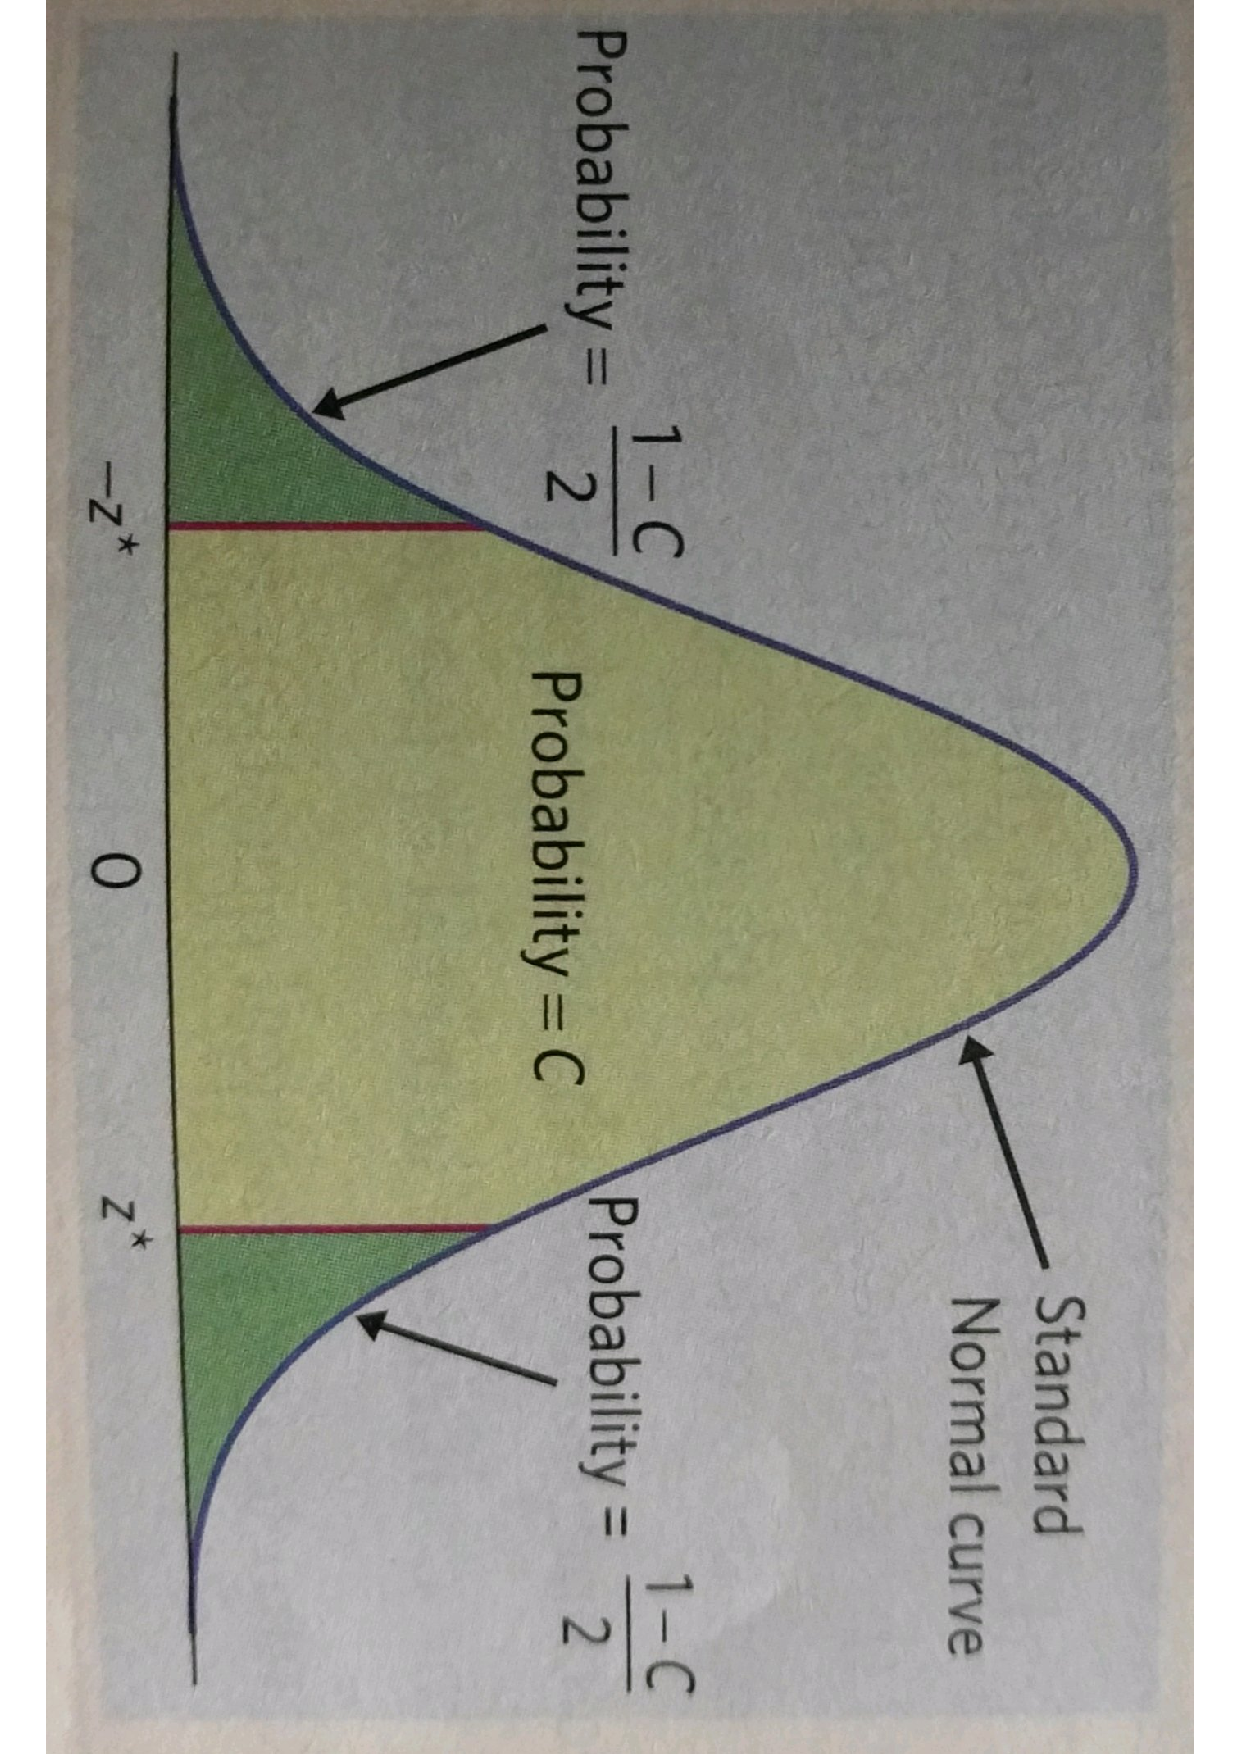
\includegraphics[scale=0.15, angle=90]{normal.pdf}
				\caption{\small The critical value $z^\star$ is the number that catches central probability $\mathcal{C}$ under a standard normal $\mathcal{N}(0,1)$ curve between $-z^\star$ and $z^\star$}
			\end{figure}
		\end{column}
		\begin{column}{0.5\textwidth}  %%<--- here
			\scriptsize
			We can use this probability statement about the \underline{standardized version} of the sample mean
			$(\bar{y} - \mu )/ \sigma / \sqrt{n}$, to place bounds on where we think the true mean lies
			by examining the probability that $\bar{y}$ is within
			$z^\star \cdot \frac{\sigma}{\sqrt{n}}$ of $\mu$ \\ 
			\begin{align*}
			\mathcal{C} & = P\left(-z^\star \le \frac{\bar{y}-\mu}{\sigma/\sqrt{n}} \le
			z^\star\right)\\
			& = P\left(-z^\star\frac{\sigma}{\sqrt{n}}
			\le \bar{y}-\mu \le +z^\star\frac{\sigma}{\sqrt{n}}\right)\\	
			& = P\left(-\bar{y}-z^\star\frac{\sigma}{\sqrt{n}} \le
			-\mu \le -\bar{y}+z^\star\frac{\sigma}{\sqrt{n}}\right)\\ 
			& = P\left(\bar{y}+z^\star\frac{\sigma}{\sqrt{n}} \ge
			\mu \ge \bar{y}-z^\star\frac{\sigma}{\sqrt{n}}\right)\\ 
			& = P\left(\bar{y}-z^\star\frac{\sigma}{\sqrt{n}} \le \mu
			\le \bar{y}+z^\star\frac{\sigma}{\sqrt{n}}\right)\\
			& = 1-\alpha
			\end{align*}
			
			We call the interval
			$\left(\bar{y}-z^\star\frac{\sigma}{\sqrt{n}},
			\bar{y}+z^\star\frac{\sigma}{\sqrt{n}}\right)$ a \textbf{(1-$\alpha$)100\%
				confidence interval} for $\mu$.
		\end{column}
	\end{columns}
	
	
}

\end{frame}







\begin{frame}[fragile]{Confidence intervals for depths of the ocean}

\vspace*{-0.19in}


\begin{knitrout}\scriptsize
\definecolor{shadecolor}{rgb}{0.969, 0.969, 0.969}\color{fgcolor}\begin{figure}

{\centering 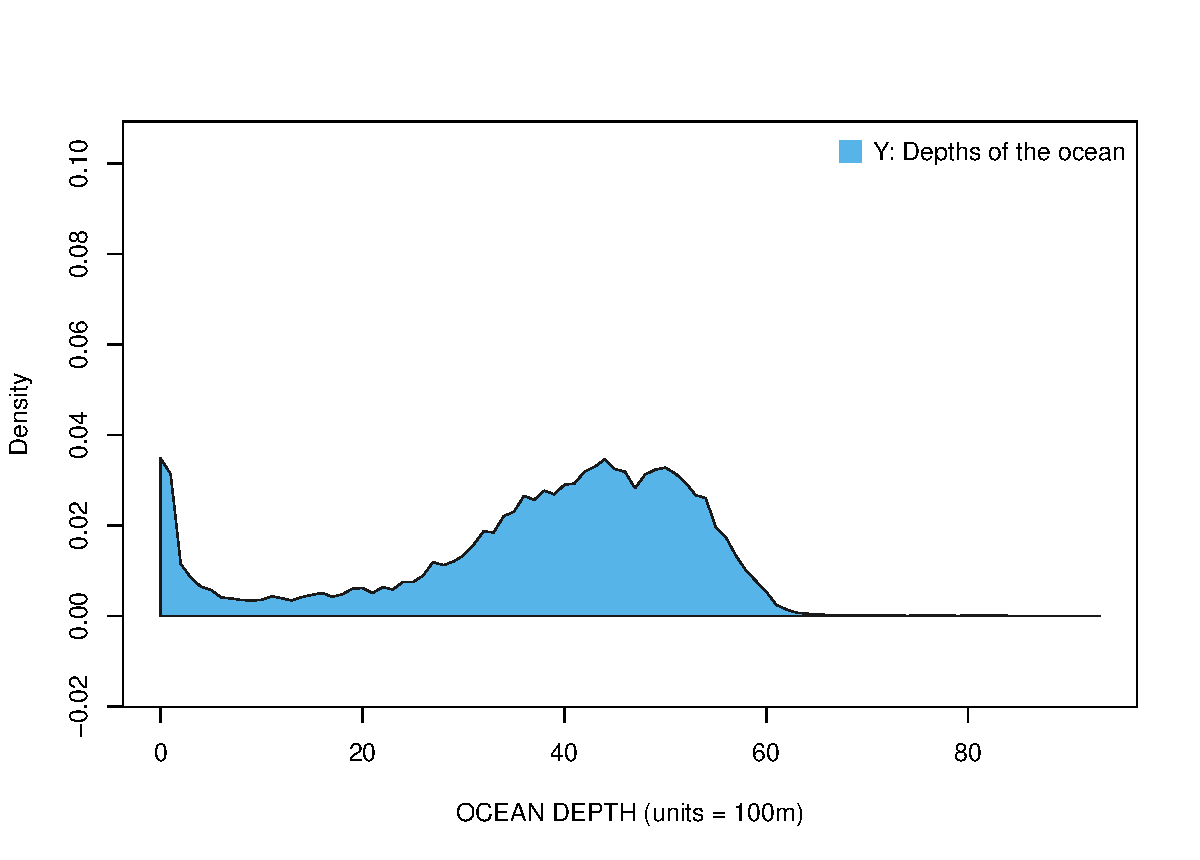
\includegraphics[width=1\linewidth]{figure/unnamed-chunk-2-1} 

}

\caption[The original data distribution of sampled depths of the ocean]{The original data distribution of sampled depths of the ocean. Note that it has multiple modes and not Normal looking.}\label{fig:unnamed-chunk-2}
\end{figure}


\end{knitrout}


\end{frame}



\begin{frame}[fragile]{The CLT is 'kicking in' at $n=16$}

\vspace*{-0.09in}


\begin{knitrout}\scriptsize
\definecolor{shadecolor}{rgb}{0.969, 0.969, 0.969}\color{fgcolor}\begin{figure}

{\centering 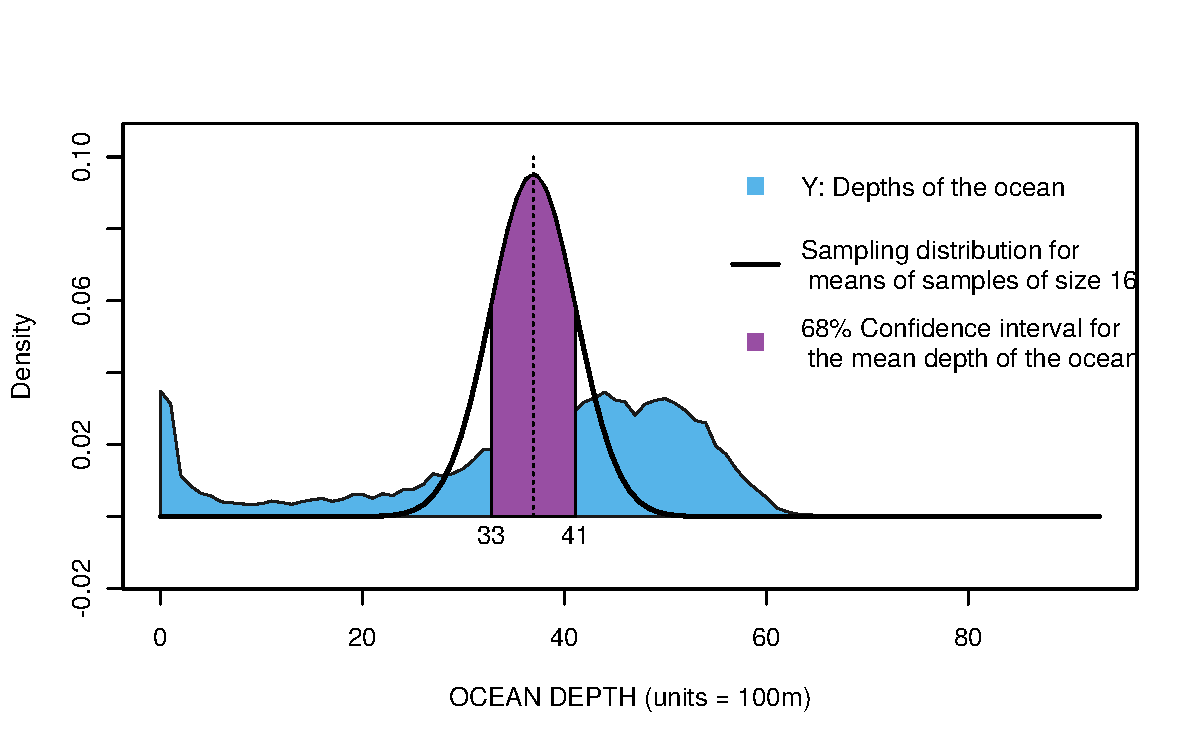
\includegraphics[width=1\linewidth]{figure/unnamed-chunk-3-1} 

}

\caption[The sampling distribution for the mean depth of the ocean with samples of size $n=16$, looks normal (centered at $\mu=37$ and SD equal to $\sigma/\sqrt{16}$) ]{The sampling distribution for the mean depth of the ocean with samples of size $n=16$, looks normal (centered at $\mu=37$ and SD equal to $\sigma/\sqrt{16}$) }\label{fig:unnamed-chunk-3}
\end{figure}


\end{knitrout}

\end{frame}


\begin{frame}[fragile]{Since CLT has 'kicked in', we use it to construct a CI}
\small
We want to construct a $\mathcal{C} = 95\%$ confidence interval for the mean. Level of significance is $\alpha = 1-\mathcal{C} = 0.05$ \pause

\begin{enumerate}
	\setlength\itemsep{1em}
	\item by the CLT $\to$ $\bar{y} \sim \mathcal{N}(mean = 37, sd = \sigma/\sqrt{16} = 4.2)$ \pause
	\item The critical value $z^\star$ such that $P(Z < -z^\star) = P(Z > z^\star) = \alpha/2 = 0.025$ is given by 
\begin{knitrout}\scriptsize
\definecolor{shadecolor}{rgb}{0.969, 0.969, 0.969}\color{fgcolor}
\begin{alltt}
\hlstd{mosaic}\hlopt{::}\hlkwd{xqnorm}\hlstd{(}\hlkwc{p} \hlstd{=} \hlkwd{c}\hlstd{(}\hlnum{0.025}\hlstd{,} \hlnum{0.975}\hlstd{))}
\end{alltt}


{\centering 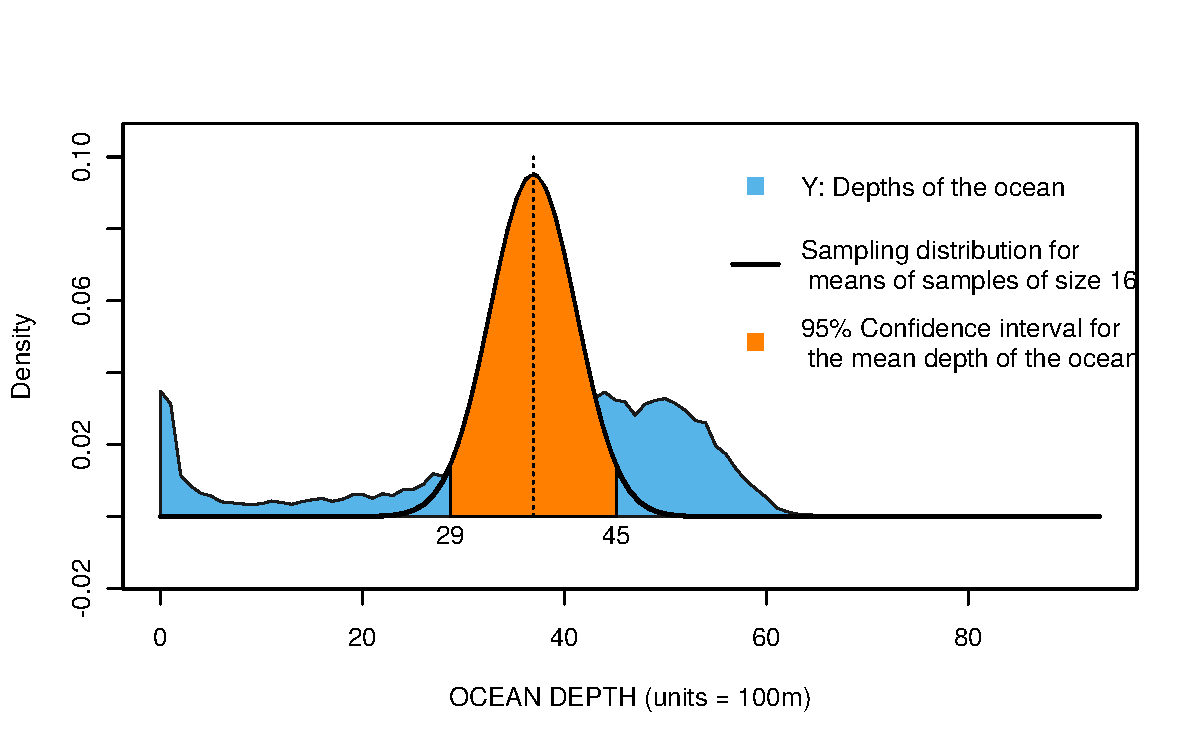
\includegraphics[width=1\linewidth]{figure/unnamed-chunk-4-1} 

}


\begin{verbatim}
## [1] -1.959964  1.959964
\end{verbatim}

\end{knitrout}
	\pause
	\item 95\% CI for $\mu$: $(37 - 1.96 \cdot 4.2, 37 + 1.96 \cdot 4.2) = [29, 45]$
\end{enumerate}
\end{frame}


\begin{frame}{Alternative way of calculating CI with CLT: \texttt{qnorm}}

\begin{itemize}
	\setlength\itemsep{1em}
	\item In the previous slides we used the standard normal $\mathcal{N}(0, 1)$ to calculate the critical value $z^\star$ needed for the CI
	\item We were able to use the $\mathcal{N}(0,1)$ for two reasons: \pause
	\begin{enumerate}
		\item the CLT \pause 
		\item the formula used to calculate the CI is based on standardizing $\bar{y} \to \frac{\bar{y} - \mu}{\sigma / \sqrt{n}}$
	\end{enumerate}
\end{itemize}
\pause 

\begin{itemize}
		\setlength\itemsep{1em}
	\item There is an alternative, \textbf{yet equivalent}, way to calculate the CI without standardizing $\bar{y}$, and without using the $\pm$ formula \pause
	\item This is accomplished using \texttt{qnorm} \pause 
	\item Note: we \textbf{still need the CLT regardless} of whether we use the $\pm$ formula or \texttt{qnorm}
\end{itemize}

\end{frame}


\begin{frame}[fragile]{68\% Confidence interval using \texttt{qnorm}}

\vspace*{-0.09in}

\Wider[2em]{
\begin{knitrout}\scriptsize
\definecolor{shadecolor}{rgb}{0.969, 0.969, 0.969}\color{fgcolor}\begin{figure}

{\centering 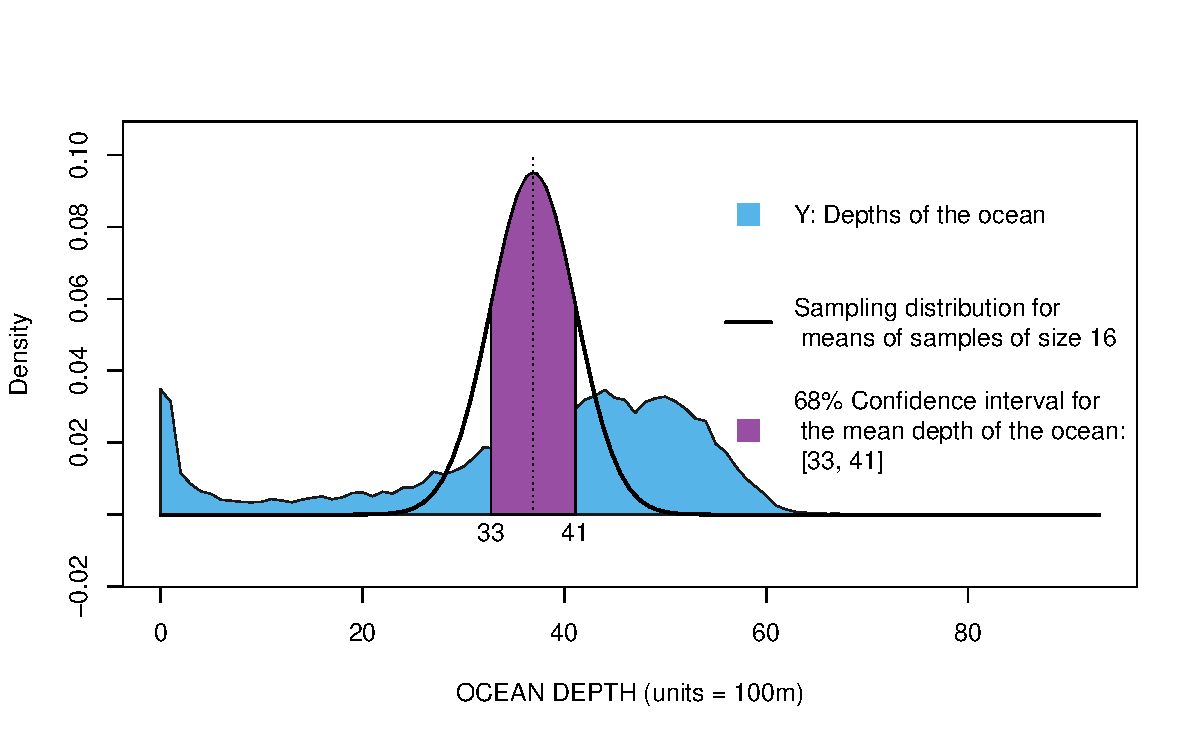
\includegraphics[width=1\linewidth]{figure/unnamed-chunk-5-1} 

}

\caption{68\% Confidence interval calculated using  \mbox{\texttt{qnorm(p = c(0.16,0.84), mean = 37, sd = 4.2)}}}\label{fig:unnamed-chunk-5}
\end{figure}


\end{knitrout}

}
\end{frame}



\begin{frame}[fragile]{95\% Confidence interval using \texttt{qnorm}}

\vspace*{-0.09in}


\Wider[2em]{
\begin{knitrout}\scriptsize
\definecolor{shadecolor}{rgb}{0.969, 0.969, 0.969}\color{fgcolor}\begin{figure}

{\centering 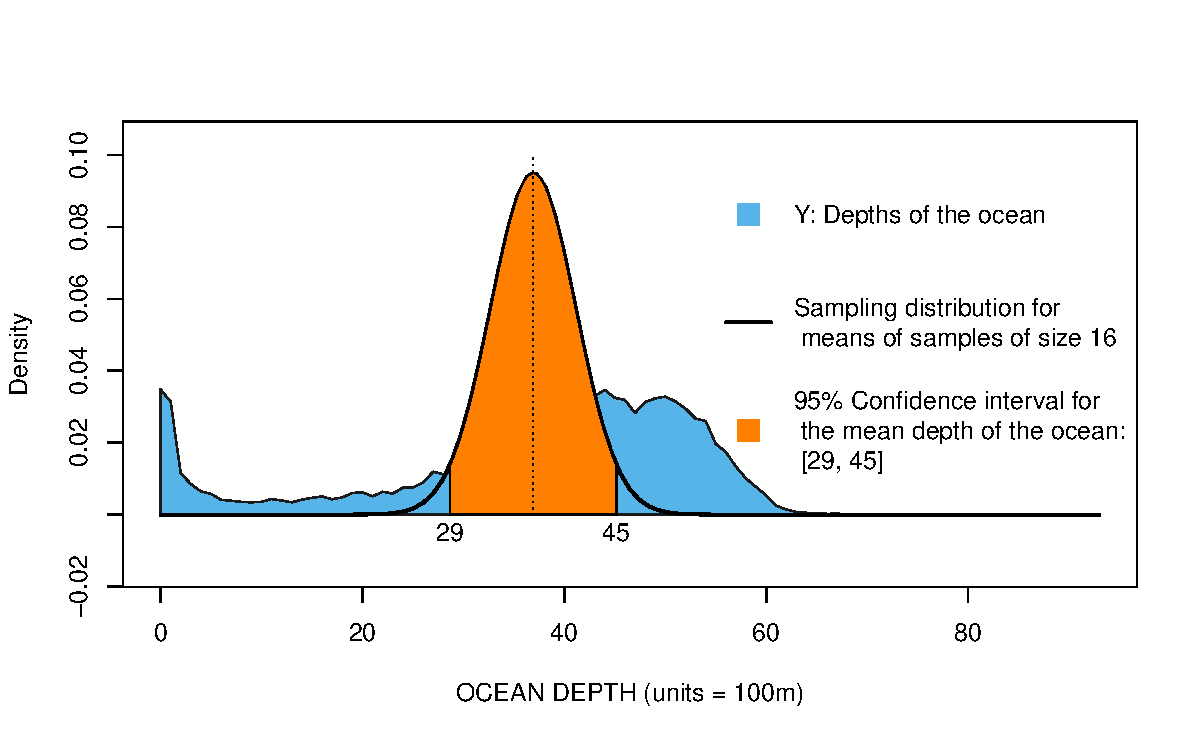
\includegraphics[width=1\linewidth]{figure/unnamed-chunk-6-1} 

}

\caption{95\% Confidence interval calculated using  \mbox{\texttt{qnorm(p = c(0.025,0.975), mean = 37, sd = 4.2)}}}\label{fig:unnamed-chunk-6}
\end{figure}


\end{knitrout}
	
}

\end{frame}


\begin{frame}{Motivation for the Bootstrap}
\begin{itemize}
	\setlength\itemsep{2em}
	\item The $\pm$ and \texttt{qnorm} methods to calculate a CI both require the CLT
\end{itemize}

\pause

\vspace*{0.2in}

\Large \textcolor{myblue}{Q: What happens if the CLT hasn't `kicked in`? Or you don't believe the CLT?} \\ \ \\
\pause 
\Large \textcolor{red}{A: Bootstrap} \\ \ \\
\end{frame}


\section{The Bootstrap}


\begin{frame}[fragile]{Ideal world: known sampling distribution}

\begin{knitrout}\scriptsize
\definecolor{shadecolor}{rgb}{0.969, 0.969, 0.969}\color{fgcolor}\begin{figure}

{\centering 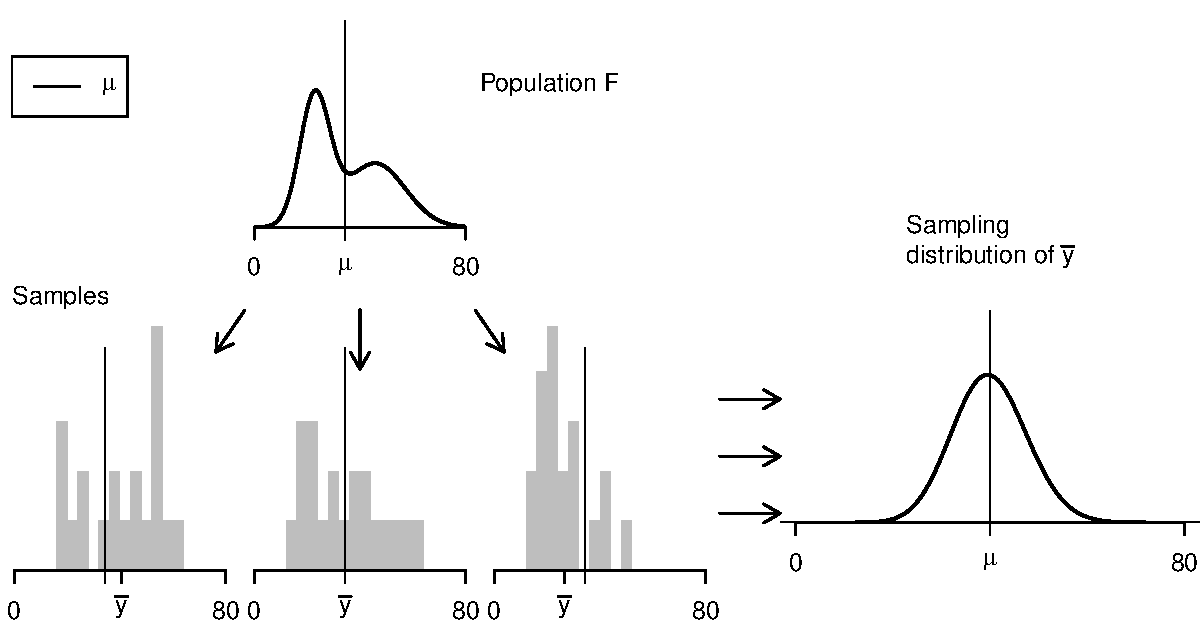
\includegraphics[width=1\linewidth]{figure/unnamed-chunk-7-1} 

}

\caption{\scriptsize{Ideal world. Sampling distributions are obtained by drawing repeated samples from the population, computing the statistic of interest for each, and collecting (an infinite number of) those statistics as the sampling distribution}}\label{fig:unnamed-chunk-7}
\end{figure}


\end{knitrout}

\end{frame}



\begin{frame}[fragile]{Reality: use the bootstrap distribution instead}




\framedgraphiccaption{boot_diag.pdf}{\scriptsize{Bootstrap world. The bootstrap distribution is obtained by drawing repeated samples from an estimate of the population, computing the statistic of interest for each, and collecting those statistics. The distribution is centered at the observed statistic ($\bar{y}$), not the parameter ($\mu$).}}

\end{frame}


\begin{frame}[fragile]{Main idea: simulate your own sampling distribution}



\begin{knitrout}\scriptsize
\definecolor{shadecolor}{rgb}{0.969, 0.969, 0.969}\color{fgcolor}
\begin{alltt}
\hlkwd{library}\hlstd{(mosaic)}
\hlstd{s_dist} \hlkwb{<-} \hlkwd{do}\hlstd{(}\hlnum{10000}\hlstd{)} \hlopt{*} \hlkwd{mean}\hlstd{(} \hlopt{~} \hlstd{alt,} \hlkwc{data} \hlstd{=} \hlkwd{resample}\hlstd{(depths.n.20))}
\hlstd{CI_95} \hlkwb{<-} \hlkwd{quantile}\hlstd{(}\hlopt{~} \hlstd{mean,} \hlkwc{data} \hlstd{= s_dist,} \hlkwc{probs} \hlstd{=} \hlkwd{c}\hlstd{(}\hlnum{0.025}\hlstd{,} \hlnum{0.975}\hlstd{))}
\end{alltt}


{\centering 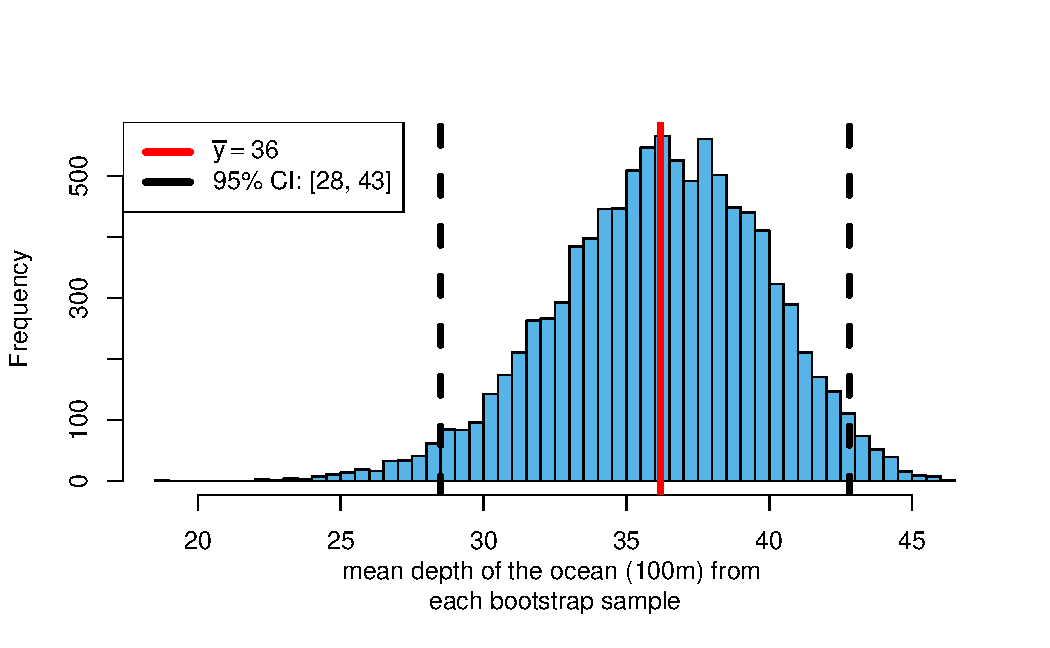
\includegraphics[width=1\linewidth]{figure/unnamed-chunk-10-1} 

}



\end{knitrout}

\end{frame}


\begin{frame}[fragile]{Bootstrap code 1}

\begin{knitrout}\scriptsize
\definecolor{shadecolor}{rgb}{0.969, 0.969, 0.969}\color{fgcolor}
\begin{alltt}
\hlcom{# function for sampling ocean depths}
\hlkwd{source}\hlstd{(}\hlstr{"https://github.com/sahirbhatnagar/EPIB607/raw/
master/exercises/water/automate_water_task.R"}\hlstd{)}

\hlcom{# from the in-class exercise}
\hlstd{index.n.20} \hlkwb{<-} \hlkwd{c}\hlstd{(}\hlnum{2106}\hlstd{,}\hlnum{2107}\hlstd{,}\hlnum{2108}\hlstd{,}\hlnum{2109}\hlstd{,}\hlnum{2110}\hlstd{,}\hlnum{2111}\hlstd{,}\hlnum{2112}\hlstd{,}
\hlnum{2113}\hlstd{,}\hlnum{2114}\hlstd{,}\hlnum{2115}\hlstd{,}\hlnum{2116}\hlstd{,}\hlnum{2117}\hlstd{,}\hlnum{2118}\hlstd{,}\hlnum{2119}\hlstd{,}
\hlnum{2120}\hlstd{,}\hlnum{2121}\hlstd{,}\hlnum{2122}\hlstd{,}\hlnum{2123}\hlstd{,}\hlnum{2124}\hlstd{,}\hlnum{2125}\hlstd{)}

\hlcom{# get depths of ocean sample n=20}
\hlstd{depths.n.20} \hlkwb{<-} \hlkwd{automate_water_task}\hlstd{(}\hlkwc{index} \hlstd{= index.n.20,}
\hlkwc{student_id} \hlstd{=} \hlnum{260194225}\hlstd{,} \hlkwc{type} \hlstd{=} \hlstr{"depth"}\hlstd{)}

\hlcom{# change to 100m units}
\hlstd{depths.n.20}\hlopt{$}\hlstd{alt} \hlkwb{=} \hlkwd{round}\hlstd{(depths.n.20}\hlopt{$}\hlstd{alt}\hlopt{/}\hlnum{100}\hlstd{,}\hlnum{0}\hlstd{)}

\hlkwd{library}\hlstd{(mosaic)}

\hlcom{# calculate mean depth for your sample}
\hlstd{mean_depth} \hlkwb{<-} \hlkwd{mean}\hlstd{(}\hlopt{~} \hlstd{alt,} \hlkwc{data} \hlstd{= depths.n.20)}
\end{alltt}

\end{knitrout}


\end{frame}

\begin{frame}[fragile]{Bootstrap code 2}

\begin{knitrout}\scriptsize
\definecolor{shadecolor}{rgb}{0.969, 0.969, 0.969}\color{fgcolor}
\begin{alltt}
\hlcom{# 10000 bootstrap samples}
\hlstd{s_dist} \hlkwb{<-} \hlkwd{do}\hlstd{(}\hlnum{10000}\hlstd{)} \hlopt{*} \hlkwd{mean}\hlstd{(} \hlopt{~} \hlstd{alt,} \hlkwc{data} \hlstd{=} \hlkwd{resample}\hlstd{(depths.n.20))}

\hlcom{# 95% CI}
\hlstd{CI_95} \hlkwb{<-} \hlkwd{quantile}\hlstd{(}\hlopt{~} \hlstd{mean,} \hlkwc{data} \hlstd{= s_dist,} \hlkwc{probs} \hlstd{=} \hlkwd{c}\hlstd{(}\hlnum{0.025}\hlstd{,} \hlnum{0.975}\hlstd{))}

\hlcom{# plot sampling distribution}
\hlkwd{hist}\hlstd{(s_dist}\hlopt{$}\hlstd{mean,} \hlkwc{breaks} \hlstd{=} \hlnum{50}\hlstd{,} \hlkwc{col} \hlstd{=} \hlstr{"#56B4E9"}\hlstd{,}
\hlkwc{main}\hlstd{=}\hlstr{""}\hlstd{,}
\hlkwc{xlab} \hlstd{=} \hlstr{"mean depth of the ocean (100m) from each bootstrap sample"}\hlstd{)}

\hlcom{# draw red line at the sample mean}
\hlkwd{abline}\hlstd{(}\hlkwc{v} \hlstd{= mean_depth,} \hlkwc{lty} \hlstd{=}\hlnum{1}\hlstd{,} \hlkwc{col} \hlstd{=} \hlstr{"red"}\hlstd{,} \hlkwc{lwd} \hlstd{=} \hlnum{4}\hlstd{)}

\hlcom{# draw black dotted lines at 95% CI}
\hlkwd{abline}\hlstd{(}\hlkwc{v} \hlstd{= CI_95[}\hlnum{1}\hlstd{],} \hlkwc{lty} \hlstd{=}\hlnum{2}\hlstd{,} \hlkwc{col} \hlstd{=} \hlstr{"black"}\hlstd{,} \hlkwc{lwd} \hlstd{=} \hlnum{4}\hlstd{)}
\hlkwd{abline}\hlstd{(}\hlkwc{v} \hlstd{= CI_95[}\hlnum{2}\hlstd{],} \hlkwc{lty} \hlstd{=}\hlnum{2}\hlstd{,} \hlkwc{col} \hlstd{=} \hlstr{"black"}\hlstd{,} \hlkwc{lwd} \hlstd{=} \hlnum{4}\hlstd{)}

\hlcom{# include legend}
\hlkwd{library}\hlstd{(latex2exp)}
\hlkwd{legend}\hlstd{(}\hlstr{"topleft"}\hlstd{,}
\hlkwc{legend} \hlstd{=} \hlkwd{c}\hlstd{(}\hlkwd{TeX}\hlstd{(}\hlstr{"$\textbackslash{}\textbackslash{}bar\{y\} = 36$"}\hlstd{),}
\hlkwd{sprintf}\hlstd{(}\hlstr{"95%% CI: [%.f, %.f]"}\hlstd{,CI_95[}\hlnum{1}\hlstd{], CI_95[}\hlnum{2}\hlstd{])),}
\hlkwc{lty} \hlstd{=} \hlkwd{c}\hlstd{(}\hlnum{1}\hlstd{,}\hlnum{1}\hlstd{),}
\hlkwc{col} \hlstd{=} \hlkwd{c}\hlstd{(}\hlstr{"red"}\hlstd{,}\hlstr{"black"}\hlstd{),} \hlkwc{lwd} \hlstd{=} \hlnum{4}\hlstd{)}
\end{alltt}

\end{knitrout}


\end{frame}

\end{document}


%%%%%%%%%%%%%%%%%%%%%%%%%%%%%%%%%%%%%%%%%%%%%%
%%%%%%%%%%%%%%%%%%%%%%%%%%%%%%%%%%%%%%%%%%%%%%
%%%%%%%%%%%%%%%%%%%%%%%%%%%%%%%%%%%%%%%%%%%%%



\begin{frame}{Examples}
\textbf{Proportions}:
	\begin{itemize}
	  \setlength\itemsep{1.2em}
	  \item Proportion of  Earth's  surface  covered  by  water
	  \item Proportion  who saw a medical doctor last year
	  \item Proportion of Québécois who don't have a family doctor
		\end{itemize}  
\pause 
	\vspace{0.1 in}
	
\textbf{Means}:
\begin{itemize}	 
	  \setlength\itemsep{1.2em} 
		\item Mean  depth  in $n$ randomly  selected  ocean  locations
		\item Mean  household  size  in $n$ randomly  selected  households.  
		\item Median  number  of  persons  under-5  in  a  sample  of $n$ households
	\end{itemize}  

\end{frame}

\frame{\frametitle{Samples must be random} 
	
\begin{itemize}
	\item 	The validity of inference will depend on the
	way that the sample was collected. If a sample was collected badly, no amount of
	statistical sophistication can rescue the study. \\ \ \\ \pause
	
	\item Samples should be \textbf{random}. That is, there should be no systematic set of
	characteristics that is related to the scientific question of interest that causes some
	people to be more likely to be sampled than others. The simplest type of randomization
	selects members from the population with equal probability (a uniform distribution). \\ \
	\\ \pause
	
	\item When conducting a study, it is always better to seek statistical
	advice sooner rather than later. Get a statistician involved at the
	\textit{planning} stage of the study... by the analysis stage, it
	may be too late!
\end{itemize}
}


\frame{\frametitle{Samples must be random - No cheating!} 
	
	\textbf{Do not cheat by} \pause 
	\begin{itemize}
		\item 	Taking 5 people from the \emph{same} household to estimate
		
		 \begin{itemize}
		 	\item proportion of Québécois who don't have a family doctor
		 	\item who saw a medical doctor last year
		 	\item average rent
		 \end{itemize}  
	 
	 \pause
	 	\vspace{0.2 in}
		
		\item Sampling the depth of the ocean \emph{only around Montreal} to estimate \begin{itemize}
			\item proportion of  Earth's  surface  covered  by  water
		\end{itemize} 

	\end{itemize}
}



\frame{\frametitle{Collecting data takes effort} 
	
	\textbf{In general} 
	\begin{itemize}
		\item The larger the sample $\to $ the more accurate the estimate (if sampling is done correctly) \pause
		
		
	\end{itemize}	
		
			 	\vspace{0.2 in}
			 	
			 		\textbf{CAVEAT} 
			 	\begin{itemize}
			 		\item Collecting more data takes effort and money!
			 		\item We will also soon discover the curse of the $\sqrt{n}$ 			 		
			 	\end{itemize}	

}


\frame{\frametitle{Collecting data takes effort} 
	
	\textbf{In general} 
	\begin{itemize}
		\item The larger the sample $\to $ the more accurate the estimate (if sampling is done correctly) \pause
		
		
	\end{itemize}	
	
	\vspace{0.2 in}
	
	\textbf{CAVEAT} 
	\begin{itemize}
		\item Collecting more data takes effort and money!
		\item We will also soon discover the curse of the $\sqrt{n}$ 			 		
	\end{itemize}	
	
}



\section{Sampling Distributions}


\frame{\frametitle{Sampling Distributions} 
	
	\begin{itemize}
				  \setlength\itemsep{2em} 
		\item Given a sample of $n$ observations from a population, we will be
		calculating estimates of the population mean, proportion, standard
		deviation, and various other population characteristics
		(parameters) \pause
		
	\item Prior to obtaining data, there is uncertainty as to which of all
		possible samples will occur \pause

\item  Because of this, estimates such as $\bar{y}$ (the sample mean) will vary
		from one sample to another
		
		
	\end{itemize}	

	
}


\frame{\frametitle{Sampling Distributions} 
	
	\begin{itemize}
		\setlength\itemsep{2em} 
		\item The behavior of such estimates in many samples of equal size is
		described by what are called \textbf{sampling distributions} \pause
		
		\item B\&M definition: The  sampling  distribution  of  a  statistic  is  the  distribution  of  values taken  by  the  statistic  in  all  possible  samples  of  the  same  size  from  the  same population.		
		
	\end{itemize}	
	
	
}

\frame{\frametitle{Why are sampling distributions important?} 
	
	\begin{itemize}
		\setlength\itemsep{2em} 
		\item They  tell  us  how  far  from  the  target  (true  value  of  the  parameter)  our  statistical  \emph{shot}  at  it  (i.e.  the  statistic  calculated  form  a  sample)  is  likely  to  be,  or, to  have  been.  \pause 
		
		\item Thus,  they  are  used  in  confidence  intervals  for  parameters. Specific  sampling  distributions  (based  on  a null value  for  the  parameter)  are also  used  in  statistical  tests  of  hypotheses.
		
	\end{itemize}	
	
	
}


\frame{\frametitle{Exercise 1: How Deep is the Ocean?} 
	
	\begin{itemize}
		\setlength\itemsep{2em} 
		\item We will get a sense of what a sampling distribution is in Exercise 1 \pause
		
		\item \textbf{CAVEAT}: This is a luxury using a toy example. In actual studies, we only get one shot!
		
	\end{itemize}	
	
	
}


\section{Exercise 1 Results}

\begin{frame}[fragile]{Sampling distribution: proportion covered by water}

\begin{knitrout}\scriptsize
\definecolor{shadecolor}{rgb}{0.969, 0.969, 0.969}\color{fgcolor}


{\ttfamily\noindent\bfseries\color{errorcolor}{\#\# Error in file(file, "{}rt"{}): cannot open the connection}}

{\ttfamily\noindent\bfseries\color{errorcolor}{\#\# Error in eval(expr, envir, enclos): object 'water\_results' not found}}

{\ttfamily\noindent\bfseries\color{errorcolor}{\#\# Error in eval(expr, envir, enclos): object 'water\_results' not found}}

{\ttfamily\noindent\bfseries\color{errorcolor}{\#\# Error in nrow(water\_results): object 'water\_results' not found}}
\end{knitrout}


\begin{knitrout}\scriptsize
\definecolor{shadecolor}{rgb}{0.969, 0.969, 0.969}\color{fgcolor}


{\ttfamily\noindent\bfseries\color{errorcolor}{\#\# Error in table(water\_results[, "{}PropnW.5.locations"{}]): object 'water\_results' not found}}

{\ttfamily\noindent\bfseries\color{errorcolor}{\#\# Error in int\_abline(a = a, b = b, h = h, v = v, untf = untf, ...): plot.new has not been called yet}}

{\ttfamily\noindent\bfseries\color{errorcolor}{\#\# Error in text.default(0.72, 40, expression(mu)): plot.new has not been called yet}}

{\ttfamily\noindent\bfseries\color{errorcolor}{\#\# Error in text.default(0.76, 41, "{}=0.71"{}): plot.new has not been called yet}}

{\ttfamily\noindent\bfseries\color{errorcolor}{\#\# Error in table(water\_results[, "{}PropnW.20.locations"{}]): object 'water\_results' not found}}

{\ttfamily\noindent\bfseries\color{errorcolor}{\#\# Error in int\_abline(a = a, b = b, h = h, v = v, untf = untf, ...): plot.new has not been called yet}}

{\ttfamily\noindent\bfseries\color{errorcolor}{\#\# Error in text.default(0.72, 40, expression(mu)): plot.new has not been called yet}}

{\ttfamily\noindent\bfseries\color{errorcolor}{\#\# Error in text.default(0.76, 41, "{}=0.71"{}): plot.new has not been called yet}}
\end{knitrout}

\end{frame}



\begin{frame}[fragile]{Sampling distribution: proportion covered by water}

\begin{knitrout}\scriptsize
\definecolor{shadecolor}{rgb}{0.969, 0.969, 0.969}\color{fgcolor}


{\ttfamily\noindent\bfseries\color{errorcolor}{\#\# Error in eval(lhs, parent, parent): object 'water\_results' not found}}

{\ttfamily\noindent\bfseries\color{errorcolor}{\#\# Error in subset(m.melt, type \%in\% c("{}Mean.20.depths"{}, "{}Mean.5.depths"{})): object 'm.melt' not found}}

{\ttfamily\noindent\bfseries\color{errorcolor}{\#\# Error in subset(m.melt, type \%in\% c("{}PropnW.20.locations"{}, "{}PropnW.5.locations"{})): object 'm.melt' not found}}
\end{knitrout}


\begin{knitrout}\scriptsize
\definecolor{shadecolor}{rgb}{0.969, 0.969, 0.969}\color{fgcolor}


{\ttfamily\noindent\bfseries\color{errorcolor}{\#\# Error in gf\_ingredients(formula = gformula, data = data, gg\_object = object, : object 'm.melt.props' not found}}
\end{knitrout}

\end{frame}



\begin{frame}[fragile]{Sampling distribution: mean depth of the ocean}


\begin{knitrout}\scriptsize
\definecolor{shadecolor}{rgb}{0.969, 0.969, 0.969}\color{fgcolor}


{\ttfamily\noindent\bfseries\color{errorcolor}{\#\# Error in hist(water\_results[, "{}Mean.5.depths"{}], xlim = c(0, 6000), ylim = c(0, : object 'water\_results' not found}}

{\ttfamily\noindent\bfseries\color{errorcolor}{\#\# Error in int\_abline(a = a, b = b, h = h, v = v, untf = untf, ...): plot.new has not been called yet}}

{\ttfamily\noindent\bfseries\color{errorcolor}{\#\# Error in text.default(3800, 45, expression(mu)): plot.new has not been called yet}}

{\ttfamily\noindent\bfseries\color{errorcolor}{\#\# Error in text.default(4100, 46, "{}=3700m"{}): plot.new has not been called yet}}

{\ttfamily\noindent\bfseries\color{errorcolor}{\#\# Error in hist(water\_results[, "{}Mean.20.depths"{}], xlim = c(0, 6000), ylim = c(0, : object 'water\_results' not found}}

{\ttfamily\noindent\bfseries\color{errorcolor}{\#\# Error in int\_abline(a = a, b = b, h = h, v = v, untf = untf, ...): plot.new has not been called yet}}

{\ttfamily\noindent\bfseries\color{errorcolor}{\#\# Error in text.default(3800, 45, expression(mu)): plot.new has not been called yet}}

{\ttfamily\noindent\bfseries\color{errorcolor}{\#\# Error in text.default(4100, 46, "{}=3700m"{}): plot.new has not been called yet}}
\end{knitrout}

\end{frame}



\begin{frame}[fragile]{Sampling distribution: mean depth of the ocean}


\begin{knitrout}\scriptsize
\definecolor{shadecolor}{rgb}{0.969, 0.969, 0.969}\color{fgcolor}


{\ttfamily\noindent\bfseries\color{errorcolor}{\#\# Error in gf\_ingredients(formula = gformula, data = data, gg\_object = object, : object 'm.melt.means' not found}}
\end{knitrout}

\end{frame}




%\begin{frame}[fragile]{Emulating the ``population''}




%\end{frame}



%\begin{frame}[fragile]{Emulating the ``population''}




%\end{frame}




\begin{comment}
\begin{frame}


The bigger the individual variaiton 

1) Normal curves. Show the 

2) the variance of y bar is the sum of the individual variances
standard error always have a root of n in the bottom

for now use 2.. estimate the sigma... Baldi and Moore give the sigma which makes no sense. 
what are the sample sizes..

start by asking 1+/- the SE, then +- 2 * SE, 
temperature in montreal for motivating the 100\%   confidence interval, 
temperature in august over the past 100 years, whos been here in montreal 0 years, 5
any one estimate has 0\% confidence


\end{frame}
\end{comment}


\section{Normal Curves and Calculations}


\subsection{Normal distribution}
\frame{\frametitle{The Normal (Gaussian) distribution} What is
	it?
	\begin{itemize}
		\item A distribution that describes continuous (numerical) data
		\item Can also be used to approximate discrete data distributions
		\item Range is (technically) infinite, though the probability of seeing
		very large or very small values is extremely tiny
		\item Fully described by only two parameters, the mean and variance
		($\mu$ and $\sigma^2$)
		\item \textcolor{red}{NOTE:} Baldi \& Moore (and \texttt{R}) use the short-hand: $X \sim
		\mathcal{N}(\mu,\sigma)$, denoting the normal distribution as a
		function of the mean and \textit{standard deviation}. This is not
		standard; many texts instead write $X \sim
		\mathcal{N}(\mu,\sigma^2)$. Be careful of this!
	\end{itemize}
} \frame{\frametitle{The Normal (Gaussian) distribution} Carl Gauss
	was a German mathematician who developed a number of important
	advances in statistics such as the method of least squares.
	\begin{figure}
		\begin{center}
			\epsfig{figure=Part2Figs/GaussMoney.eps,width=3.2in,height=2.5in}
		\end{center}
	\end{figure}
} 

\frame{\frametitle{The Normal distribution} Where do Normal data
	come from?
	\begin{itemize}
		\item Natural processes
		\begin{itemize}
			\item Blood pressure
			\item Height
			\item Weight
			\item[]
		\end{itemize} \pause
		\item ``Man-made'' (or derived)
		\begin{itemize}
			\item Binomial (proportion) and Poisson (count) data are
			approximately Normal under certain conditions
			\item Sums and means of random variables (Central Limit Theorem)
			\item Data can sometimes be made to look Normal via transformations
			(squares, logs, etc)
		\end{itemize}
	\end{itemize}
} 

\frame{\frametitle{The Normal distribution} For Normal data, we
	can use \sout{the Gaussian tables} \texttt{R} to answer the questions:
	\begin{itemize}
		\item What is the probability that a single observation $X$ is
		\begin{itemize}
			\item greater than $X^*$?
			\item less than $X^*$?
			\item between $X^*_L$ and $X^*_U$?
		\end{itemize}
		\item That is, we can find out information about the percent
		distribution of $X$ as a function of thresholds $X^*$, or $X^*_L$
		and $X^*_U$.
		\item[] \pause
		\item We can also use \sout{the Normal tables} \texttt{R} to find out information about
		thresholds $X^*$ that will contain particular percentages of
		the data. I.e., we can find what threshold values will
		\begin{itemize}
			\item Exclude the lower $\omega^*$\% of a population
			\item Exclude the upper $\omega^*$\% of a population
			\item Contain the middle $\omega^*$\% of a population
		\end{itemize}
	\end{itemize}
}

\frame{\frametitle{The Normal distribution} We can use \sout{the
	Gaussian tables} \texttt{R} to answer these questions \textbf{no matter
		what the values
		of} $\mu$ and $\sigma^2$. \\ \ \\
	That is, the \% of the Normal distribution falling between $X^*_L =
	\mu - m_1\sigma$ and $X^*_U = \mu + m_2\sigma$ where
	$m_1, m_2$ are any multiples \textbf{remains the same} for any $\mu$ and $\sigma$. \\ \ \\
	How so?? \pause
	\begin{center}
		Because we can \textbf{standardize} any $X \sim
		\mathcal{N}(\mu,\sigma)$ to find $Z \sim \mathcal{N}(0,1)$
\end{center} }

\frame{\frametitle{The Normal distribution} An illustration
	using IQ scores, which we presume have a $\mathcal{N}(100,13)$
	distribution of scores. \\ \ \\
	
	\textcolor{blue}{Q1:} What percentage of scores are
	\textbf{above}
	130? \\
	Two steps:
	\begin{enumerate}
		\item Change of location from $\mu_X=100$ to $\mu_Z=0$
		\item Change of scale from $\sigma_X=13$ to $\sigma_Z=1$
		\item[]
	\end{enumerate}
	Together, this gives us \[Z = \frac{X-\mu_X}{\sigma_X} =
	\frac{130-100}{13} = 2.31\] }

\begin{frame}[fragile]{The Normal distribution}

\vspace*{-.01in}

\small{The position of $X$=130 in a $\mathcal{N}(100,13)$ distribution is the same as
the place of $Z=2.31$ on the $\mathcal{N}(0,1)$, which we call the \textbf{standardized} Normal distribution (or	$Z$-distribution).}
	
	%\begin{figure}
%		\begin{center}
%			\epsfig{figure=Part1Figs/TwoNormals-equalProb.eps,width=4.4in,height=2.5in}
%		\end{center}
%	\end{figure}

\begin{knitrout}\scriptsize
\definecolor{shadecolor}{rgb}{0.969, 0.969, 0.969}\color{fgcolor}

{\centering 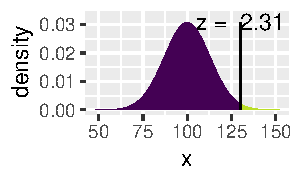
\includegraphics[width=0.55\linewidth]{figure/probs-1} 

}




{\centering 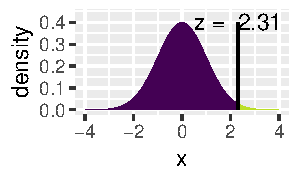
\includegraphics[width=0.55\linewidth]{figure/probs-2} 

}



\end{knitrout}

\end{frame} 

\frame{\frametitle{The Normal distribution} How are the
	values
	in the Normal tables found?\\ \ \\
	Normal density:
	\[f(x|\mu,\sigma) = \frac{1}{\sqrt{2\pi}\sigma}\exp\frac{-(x-\mu)^2}{2\sigma^2}\]
	
	\vspace{.5cm} Probabilities found by integration (area under the
	Normal curve): \[ P(a \le x \le b) =
	\int_a^b\frac{1}{\sqrt{2\pi}\sigma}\exp\frac{-(x-\mu)^2}{2\sigma^2}dx\]
}


\frame{\frametitle{The Normal distribution} (The percent above
	$X=130$) = (\% above $Z=2.31$) =1.04\%\\ \ \\
	
	How do we know this? We look at the lower tail probability of
	2.31 [i.e., the \% below 2.31], and then subtract it from 1:
	\begin{enumerate}
		\item $P(X < 130) = P(Z < 2.31) = 0.9896$
		\item $P(X > 130) = 1 - P(X < 130) = 0.0104$
		\item[]
	\end{enumerate}
	So 130 is the 98.96$^{th}$ percentile of a $\mathcal{N}$(100,13)
	distribution. }


\begin{frame}{Reminder about percentiles and quantiles}

\begin{itemize}
	\item \textbf{Quantile}
	\begin{itemize}
		\item Any set of data, arranged in ascending or descending order, can be divided into various parts, also known as partitions or subsets, regulated by quantiles. 
		\item Quantile is a generic term for those values that divide the set into partitions of size $n$, so that each part represents $1/n$ of the set. 
		\item Quantiles are not the partition itself. They are the numbers that define the partition. 
		\item You can think of them as a sort of numeric boundary.
	\end{itemize}
\end{itemize}
\pause 

\begin{itemize}
	\item \textbf{Percentile}
	\begin{itemize}
		\item Percentiles are quite similar to quantiles: they split your set, but only into two partitions. 
		\item For a generic $k$th percentile, the lower partition contains k\% of the data, and the upper partition contains the rest of the data, which amounts to 100 - k \%, because the total amount of data is 100\%. 
		\item Of course k can be any number between 0 and 100.
	\end{itemize}
\end{itemize}

\end{frame}



\begin{frame}{More about percentiles and quantiles}
\begin{itemize}
	\item In class, we will find ourselves asking for the quantiles of a distribution. 
	\item Percentiles go from 0 to 100
	\item Quantiles go from any number to any number
	\item Percentiles are examples of quantiles and you might find some people use them interchangeably (though this may not always be correct since quantiles can take on any value, positive or negative). 
	\item \textbf{In particular}, \texttt{R} uses the term quantiles. 
	%\item This is a small semantic quibble, but we ought to be precise. 
	%\item That being said, I won't correct somebody if they call these percentiles. 
	\item \textcolor{blue}{In the previous example}, we saw that $P(Z < 2.31) = 0.9896$. In \texttt{R}, 2.31 is called the quantile 
	.
\end{itemize}
\end{frame}


\frame{\frametitle{The Normal distribution} (The percent above
	$X=130$) = (\% above $Z=2.31$) =1.04\%\\ \ \\
	
	But wait!! The standard Normal is symmetric about 0, so we can do
	this another way... The \% \textbf{above} 2.31 is equal to the \%
	\textbf{below} -2.31:
	\begin{itemize}
		\item[] $P(X > 130) = P(Z > 2.31)$ \pause
		\item[] $\qquad \Rightarrow$ $P(Z > 2.31) = P(Z < -2.31) $ \pause
		\item[] $\qquad \Rightarrow$ $P(X > 130) = P(Z < -2.31) = 0.0104$
		\item[]
	\end{itemize}
	So 130 is the 98.96$^{th}$ percentile of a $\mathcal{N}(130,13)$ distribution. What is
	the 1.04$^{th}$ percentile? \\ \ \\\pause
	
	Transform from $Z = -2.31$ back to $X$:
	\[ X = \sigma Z + \mu = 13(-2.31) + 100 = 69.97.\]
	
}

\begin{frame}[fragile]{For probabilities we use $pnorm$}


\begin{knitrout}\scriptsize
\definecolor{shadecolor}{rgb}{0.969, 0.969, 0.969}\color{fgcolor}
\begin{alltt}
\hlstd{stats}\hlopt{::}\hlkwd{pnorm}\hlstd{(}\hlkwc{q} \hlstd{=} \hlnum{130}\hlstd{,} \hlkwc{mean} \hlstd{=} \hlnum{100}\hlstd{,} \hlkwc{sd} \hlstd{=} \hlnum{13}\hlstd{)}
\end{alltt}
\begin{verbatim}
## [1] 0.9894919
\end{verbatim}

\end{knitrout}

\pause 

\begin{knitrout}\scriptsize
\definecolor{shadecolor}{rgb}{0.969, 0.969, 0.969}\color{fgcolor}
\begin{alltt}
\hlstd{mosaic}\hlopt{::}\hlkwd{xpnorm}\hlstd{(}\hlkwc{q} \hlstd{=} \hlnum{130}\hlstd{,} \hlkwc{mean} \hlstd{=} \hlnum{100}\hlstd{,} \hlkwc{sd} \hlstd{=} \hlnum{13}\hlstd{)}
\end{alltt}


{\centering 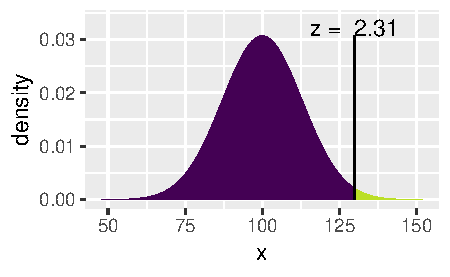
\includegraphics[width=0.6\linewidth]{figure/probs3-1} 

}


\begin{verbatim}
## [1] 0.9894919
\end{verbatim}

\end{knitrout}

\pause 

\begin{itemize}
	\item \texttt{pnorm} returns the integral from $-\infty$ to $q$ for a $\mathcal{N}(\mu, \sigma)$
	\item \texttt{pnorm} goes from \textit{quantiles} (think $Z$ scores) to probabilities
\end{itemize}

\end{frame}



\begin{frame}[fragile]{For quantiles we use $qnorm$}



\begin{knitrout}\scriptsize
\definecolor{shadecolor}{rgb}{0.969, 0.969, 0.969}\color{fgcolor}
\begin{alltt}
\hlstd{stats}\hlopt{::}\hlkwd{qnorm}\hlstd{(}\hlkwc{p} \hlstd{=} \hlnum{0.0104}\hlstd{,} \hlkwc{mean} \hlstd{=} \hlnum{100}\hlstd{,} \hlkwc{sd} \hlstd{=} \hlnum{13}\hlstd{)}
\end{alltt}
\begin{verbatim}
## [1] 69.94926
\end{verbatim}

\end{knitrout}

\pause 

\begin{knitrout}\scriptsize
\definecolor{shadecolor}{rgb}{0.969, 0.969, 0.969}\color{fgcolor}
\begin{alltt}
\hlstd{mosaic}\hlopt{::}\hlkwd{xqnorm}\hlstd{(}\hlkwc{p} \hlstd{=} \hlnum{0.0104}\hlstd{,} \hlkwc{mean} \hlstd{=} \hlnum{100}\hlstd{,} \hlkwc{sd} \hlstd{=} \hlnum{13}\hlstd{)}
\end{alltt}


{\centering 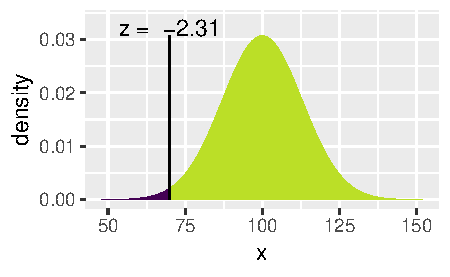
\includegraphics[width=0.6\linewidth]{figure/probs5-1} 

}


\begin{verbatim}
## [1] 69.94926
\end{verbatim}

\end{knitrout}

\pause 

\small{
\begin{itemize}
	\item \texttt{qnorm} answers the question: What is the Z-score of the $p$th percentile of the normal distribution?
		
	\item \texttt{qnorm} goes from \textit{probabilities} to quantiles 
\end{itemize}
}
\end{frame}


\frame{\frametitle{The Normal distribution}
	\textcolor{blue}{Q2:} What is the probability of seeing an IQ
	score \textbf{as extreme as} (think highly unusual)  130? \\
	\begin{enumerate}
		\item Again, we find that $X=130$ is the same percentile of the
		IQ Normal distribution as $Z=2.31$ is of the standard Normal. \pause
		\item To see what scores are as extreme, we want to know the
		probability that $Z>$2.31 or that $Z<$-2.31. \pause
		\item As we saw previously, $P(Z > 2.31) = P(Z < -2.31) =
		0.0104$, so the probability of seeing an IQ as extreme or more
		so than 130 is $2\times0.0104 = 0.0208$.
	\end{enumerate}
}


\begin{frame}[fragile]{Finding tail probabilities}



\begin{knitrout}\scriptsize
\definecolor{shadecolor}{rgb}{0.969, 0.969, 0.969}\color{fgcolor}
\begin{alltt}
\hlcom{# lower.tail = TRUE is the default}
\hlstd{stats}\hlopt{::}\hlkwd{pnorm}\hlstd{(}\hlkwc{q} \hlstd{=} \hlopt{-}\hlnum{2.31}\hlstd{,} \hlkwc{mean} \hlstd{=} \hlnum{0}\hlstd{,} \hlkwc{sd} \hlstd{=} \hlnum{1}\hlstd{,} \hlkwc{lower.tail} \hlstd{=} \hlnum{TRUE}\hlstd{)} \hlopt{+}
\hlstd{stats}\hlopt{::}\hlkwd{pnorm}\hlstd{(}\hlkwc{q} \hlstd{=} \hlnum{2.31}\hlstd{,} \hlkwc{mean} \hlstd{=} \hlnum{0}\hlstd{,} \hlkwc{sd} \hlstd{=} \hlnum{1}\hlstd{,} \hlkwc{lower.tail} \hlstd{=} \hlnum{FALSE}\hlstd{)}
\end{alltt}
\begin{verbatim}
## [1] 0.02088815
\end{verbatim}

\end{knitrout}

\pause 

\begin{knitrout}\scriptsize
\definecolor{shadecolor}{rgb}{0.969, 0.969, 0.969}\color{fgcolor}
\begin{alltt}
\hlstd{mosaic}\hlopt{::}\hlkwd{xpnorm}\hlstd{(}\hlkwc{q} \hlstd{=} \hlkwd{c}\hlstd{(}\hlopt{-}\hlnum{2.31}\hlstd{,}\hlnum{2.31}\hlstd{),} \hlkwc{mean} \hlstd{=} \hlnum{0}\hlstd{,} \hlkwc{sd} \hlstd{=} \hlnum{1}\hlstd{)}
\end{alltt}


{\centering 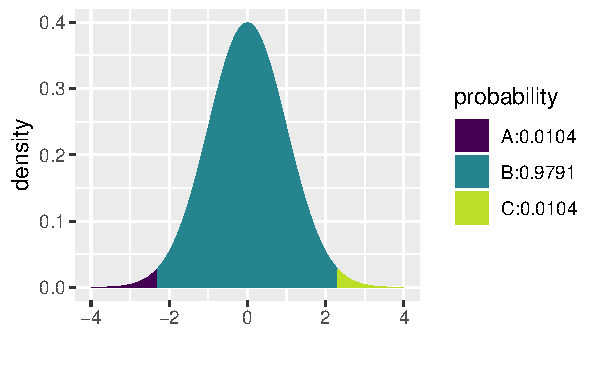
\includegraphics[width=0.6\linewidth]{figure/probs7-1} 

}


\begin{verbatim}
## [1] 0.01044408 0.98955592
\end{verbatim}

\end{knitrout}


\end{frame}



\begin{frame}[fragile]{The Normal distribution}
	\textcolor{blue}{Q3:}
	What is the 75$^{th}$ percentile of the IQ scores distribution? \\
	We now have to reverse the sequence of steps: \pause
	\begin{itemize}
		\item \textcolor{blue}{Ask yourself:} What $Z$ value corresponds to a probability of 0.75? Should you use \texttt{pnorm} or \texttt{qnorm}? \pause

\begin{knitrout}\scriptsize
\definecolor{shadecolor}{rgb}{0.969, 0.969, 0.969}\color{fgcolor}
\begin{alltt}
\hlstd{mosaic}\hlopt{::}\hlkwd{xqnorm}\hlstd{(}\hlkwc{p} \hlstd{=} \hlnum{0.75}\hlstd{,} \hlkwc{mean} \hlstd{=} \hlnum{100}\hlstd{,} \hlkwc{sd} \hlstd{=} \hlnum{13}\hlstd{)}
\end{alltt}


{\centering 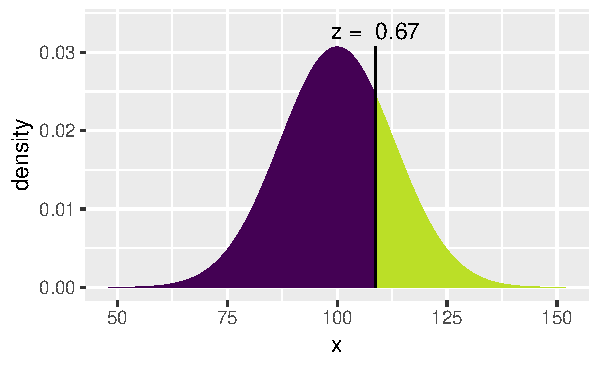
\includegraphics[width=0.6\linewidth]{figure/probs8-1} 

}


\begin{verbatim}
## [1] 108.7684
\end{verbatim}

\end{knitrout}

		\item[]
	\end{itemize} This tells us that 75\% of the IQ scores fall below 108.8. 
\end{frame}


\begin{frame}[fragile]{Empirical Rule or 68-95-99.7\% Rule}

In any normal distribution with mean $\mu$ and standard deviation $\sigma^2$:
\begin{itemize}
			\setlength\itemsep{2em}
	\item Approximately 68\% of the data fall within one standard deviation of the mean.
\item Approximately 95\% of the data fall within two standard deviations of the mean.
\item Approximately 99.7\% of the data fall within three standard deviations of the mean.
\end{itemize}
\end{frame}

\begin{frame}[fragile]{Demo of Empirical Rule}

\begin{knitrout}\scriptsize
\definecolor{shadecolor}{rgb}{0.969, 0.969, 0.969}\color{fgcolor}
\begin{alltt}
\hlstd{pacman}\hlopt{::}\hlkwd{p_load}\hlstd{(mosaic)}
\hlstd{pacman}\hlopt{::}\hlkwd{p_load}\hlstd{(manipulate)}

\hlstd{mNorm} \hlkwb{<-} \hlkwa{function}\hlstd{(}\hlkwc{mean} \hlstd{=} \hlnum{0}\hlstd{,} \hlkwc{sd} \hlstd{=} \hlnum{1}\hlstd{) \{}
  \hlstd{lo} \hlkwb{<-} \hlstd{mean} \hlopt{-} \hlnum{5} \hlopt{*} \hlstd{sd}
  \hlstd{hi} \hlkwb{<-} \hlstd{mean} \hlopt{+} \hlnum{5} \hlopt{*} \hlstd{sd}
  \hlkwd{manipulate}\hlstd{(}
        \hlkwd{xpnorm}\hlstd{(}\hlkwd{c}\hlstd{(A,B), mean, sd,} \hlkwc{verbose} \hlstd{=} \hlnum{FALSE}\hlstd{,} \hlkwc{invisible} \hlstd{=} \hlnum{TRUE}\hlstd{),}
        \hlkwc{A} \hlstd{=} \hlkwd{slider}\hlstd{(lo, hi,} \hlkwc{initial} \hlstd{= mean} \hlopt{-} \hlstd{sd),}
        \hlkwc{B} \hlstd{=} \hlkwd{slider}\hlstd{(lo, hi,} \hlkwc{initial} \hlstd{= mean} \hlopt{+} \hlstd{sd)}
 \hlstd{)}
\hlstd{\}}
\hlkwd{mNorm}\hlstd{(}\hlkwc{mean} \hlstd{=} \hlnum{0}\hlstd{,} \hlkwc{sd} \hlstd{=} \hlnum{1}\hlstd{)}
\end{alltt}

\end{knitrout}
\end{frame}


\begin{frame}[fragile]{Empirical Rule or 68-95-99.7\% Rule}

\framedgraphic{6899rule.png}

\end{frame}

\frame{\frametitle{Properties of Normal random variables} Special
	properties of the Normal distribution:
	\begin{itemize}
		\item[] \item In $Y$ is a Normal random variable, then so is $a+bY$. \pause
		\item[] \item If $X$ and $Y$ are two Normal random variables, then
		$X+Y$ is a Normal random variable. What is the mean and variance of this new random
		variable? \pause
		\item[] \item If $X$ and $Y$ are two Normal random variables and
		$\rho_{XY}=0$ (correlation between $X$ and $Y$), then $X$ and $Y$ are independent.
	\end{itemize}
} \frame{\frametitle{Properties of Normal random variables} 
	Let $Y_1,...,Y_n \sim \mathcal{N}(\mu,\sigma)$, and let each $Y_i$
	be independent of the others. (\textcolor{blue}{think simple random sample})\\ \ \\
	
	Then $\overline{Y} = \frac{1}{n}\sum_{i=1}^n Y_i$ has what distribution? \pause
	\begin{itemize}
		\item The sum of Normal random variables is Normal, so $\overline{Y}$ is a
		Normal random variable. \pause
		\item $E(\overline{Y}) = \frac{1}{n}\sum_{i=1}^n E(Y_i) =  \frac{1}{n}\sum_{i=1}^n \mu =
		\mu$.\pause
		\item $Var(\overline{Y}) = Var(\frac{1}{n}\sum_{i=1}^n Y_i) =  \frac{1}{n^2}\sum_{i=1}^n Var(Y_i) =
		\sigma^2/n$. \pause 
		\item Standard Error of $\overline{Y}$ = $\sqrt{Var(\overline{Y})} = \sigma / \sqrt{n}$
	\end{itemize}
}



\begin{comment}
\frame{\frametitle{Properties of estimators} As we have discussed,
	there are several properties that we want in an estimator:
	\begin{enumerate}
		\item Unbiased: the expected value (mean) of the estimator is equal to the
		parameter
		\begin{itemize}
			\item The sample mean, $\overline{y}$, is unbiased for the population
			mean, $\mu$
		\end{itemize} \pause
		\item Consistent: as sample size gets larger, the estimator gets
		closer to the parameter \pause
	\end{enumerate}
	How do we go about finding an estimator might have good properties?
	\\ \ \\ \pause
	
	One approach to finding good estimates is to ask ``What value of the parameter is most
	likely, given the data that I observed?'' Such an estimate is a \textbf{Maximum
		Likelihood Estimator} (MLE). } \frame{\frametitle{Maximum Likelihood Estimators} Suppose
	we have a sample $x_1,x_2,...,x_n$ from a Normally distributed population with unknown
	mean $\mu$ and known variance $\sigma^2=1$. We want to estimate $\mu$ from the data. The
	obvious estimator is the sample mean, $\bar{x}$. \\ \ \\\pause
	
	We have already shown that the sample mean is unbiased (that is,
	$E[\bar{x}] = \mu$) and that we can control its variability through
	the size of our sample (since Var$[\bar{x}] = \sigma^2/n$). Are
	there other theoretically justifications for using the sample mean?
} \frame{\frametitle{Maximum Likelihood Estimators} It turns out
	that $\bar{x}$ maximizes the probability of the observed data, given
	$\mu$. An estimator that has this property is a \textbf{maximum
		likelihood estimator}.
	\begin{figure}
		\begin{center}
			\epsfig{figure=Part2Figs/MLE-R-1.eps,width=3in,height=2.7in}
		\end{center}
	\end{figure}
} \frame{\frametitle{Maximum Likelihood Estimators} It turns out
	that $\bar{x}$ maximizes the probability of the observed data, given
	$\mu$. An estimator that has this property is a \textbf{maximum
		likelihood estimator}.
	\begin{figure}
		\begin{center}
			\epsfig{figure=Part2Figs/MLE-R-2.eps,width=3in,height=2.7in}
		\end{center}
	\end{figure}
} \frame{\frametitle{Maximum Likelihood Estimators} It turns out
	that $\bar{x}$ maximizes the probability of the observed data, given
	$\mu$. An estimator that has this property is a \textbf{maximum
		likelihood estimator}.
	\begin{figure}
		\begin{center}
			\epsfig{figure=Part2Figs/MLE-R-3.eps,width=3in,height=2.7in}
		\end{center}
	\end{figure}
} \frame{\frametitle{Maximum Likelihood Estimators} It turns out
	that $\bar{x}$ maximizes the probability of the observed data, given
	$\mu$. An estimator that has this property is a \textbf{maximum
		likelihood estimator}.
	\begin{figure}
		\begin{center}
			\epsfig{figure=Part2Figs/MLE-R-4.eps,width=3in,height=2.7in}
		\end{center}
	\end{figure}
}
content...
\end{comment}

\begin{comment}
\frame{\frametitle{Maximum Likelihood Estimators} For each data
point, the probability density function is given by:
\[ f(x_i|\mu,\sigma) = \frac{1}{\sqrt{2p}\sigma}\exp\left(-\frac{(x_i-\mu)^2}{2\sigma^2}\right). \]
Since the data are independent, we can use the product rule:
\begin{eqnarray*}
f(x_1,x_2,...,x_n|\mu,\sigma) & = &
\prod_{i=1}^n\frac{1}{\sqrt{2p}\sigma}\exp\left(-\frac{(x_i-\mu)^2}{2\sigma^2}\right)\\
& = & \frac{1}{\sqrt{2p}\sigma}\exp\left(-\frac{\sum_{i=1}^n(x_i-\mu)^2}{2\sigma^2}\right).\\
\end{eqnarray*}
This function is called a \textbf{likelihood function}; it describes
the likelihood (or the probability) of the observed data for a given
value of $\mu$ (and $\sigma$). }

\frame{\frametitle{Maximum Likelihood Estimators} We want to maximize this probability
function. That is, we want to find the value of $\mu$ that gives the highest probability
to the data we observed. \\ \ \\ \pause

From calculus, we know that we maximize a function by taking its derivative and set it
equal to zero. Doing this and simplifying gives
\[\frac{1}{2\sigma^2}\sum_{i=1}^n2(x_i-\mu) = 0.\] \pause

This implies \[\sum_{i=1}^n(x_i-\mu) = \sum_{i=1}^nx_i - n\mu  = 0\]
so that the likelihood is maximized at $\mu=
\frac{1}{n}\sum_{i=1}^nx_i = \bar{x}.$ Thus the MLE of $\mu$ is
$\bar{x}.$ }
\end{comment}

%%%%%%%%%%%%%%%%%%%%%%%%%%%%%%%%%%%%%%%%%%%%%%%%%%%%%%%%%%%%%%%%%%%
\begin{comment}
\subsection{Normal approximation to binomial}

\frame{\frametitle{Normal approximation of the binomial
		distribution} Suppose we take a large random sample of size $n$
	in our population, and count $X$, the number of `successes'
	(success could be the event of having MS, the event of
	exercising more than twice per week, etc.).
	\begin{itemize}
		\item We can view $X$ as being sampled from a Binomial$(n,p)$
		distribution... \pause
		\item OR we can view $X$ as the sum of $n$ binary variable
		$Y_1$,...,$Y_n$ where $Y_i \sim$ Binomial$(1,p)$.
		\item The Binomial$(1,p)$ distribution is also called a
		Bernoulli$(p)$ distribution.
	\end{itemize}
} \frame{\frametitle{Normal approximation of the binomial} Now
	$\hat{p} = X/n$ is the sample proportion of successes, which is an
	estimate of $p$, the mean of the Bernoulli$(p)$ distribution. \\ \ \\
	
	If $\min(np,n(1-p)) \ge 10$, then we have
	\begin{itemize}
		\item $X$ is approximately distributed $\mathcal{N}(np,\sqrt{np(1-p)})$
		\item $\hat{p}$ is approximately distributed $\mathcal{N}(\quad,\quad\quad)$
	\end{itemize}
} \frame{\frametitle{Normal approximation of the binomial}
	Why is this true? \\
	\begin{itemize}
		\item[] \item For $\hat{p}$, this is easy to explain: $\hat{p}$ is just a
		sample average of Bernoulli random variables, since \[\hat{p} = X/n =
		(\frac{1}{n}\sum_{i=1}^n Y_i),\] and so the CLT applies. \pause
		\item[] \item But what about $X$? $X$ is just a linear
		transformation of $\hat{p}$, since $X = n\hat{p}$, and linear
		combinations of (approximately) Normal random variables are
		(approximately) Normal.
		\item[] \item The approximation is best when $p$ is near 0.5 (which makes the
		distribution of $X$ symmetric) and/or $n$ is large.
	\end{itemize}
} \frame{\frametitle{Normal approximation of the binomial}
	\begin{figure}
		\begin{center}
			\epsfig{figure=Part2Figs/NormalApproxBino.eps,width=3.3in,height=3.3in}
		\end{center}
	\end{figure}
}

\frame{\frametitle{Normal approximation of the binomial}
	Suppose we collect a simple random sample of $n=150$ health
	care workers in India. What is the probability that $X=80$ or
	more of the individuals show antibody response to TB
	(indicating previous TB exposure) if $p=0.6$? \\ \ \\
	
	Our binomial tables do not cover the cases for $n$ as large as
	150. Also, calculating
	\[ P(X = 80\hbox{ out of } 150) =
	\frac{150!}{(150-80)!80!}0.6^{80}0.4^{(150-80)}\] is difficult at
	best. 150! is a number that is over 250 digits long, and $0.6^{80}$
	is very, very small. Not only that, but to find $P(X \ge 80\hbox{ out of } 150)$, we would have to sum 70
	terms to calculate this probability. }

\frame{\frametitle{Normal approximation of the binomial} Let's
	use the Normal approximation!! \\ \ \\
	First, we need to calculate the mean and variance of the
	distribution:
	\begin{eqnarray*}
		\mu & = & np = 150\times0.6 = 90\\
		\sigma^2 & = & np(1-p) = 150\times0.6\times0.4 = 36
	\end{eqnarray*} \pause
	The Normal approximation to the binomial is improved by using a
	\textbf{continuity correction}, so that instead of estimation $P(X
	\ge 80|X\sim\hbox{Bino}(150,0.6))$ we estimate $P(X \ge
	79.5|X\sim\hbox{Bino}(150,0.6))$, and approximate this by $P(X \ge
	79.5|X\sim\mathcal{N}(90,6))$. }

\frame{\frametitle{Normal approximation of the binomial}
	{\small
		\[P(X \ge 80|X\sim\hbox{Bino}(150,0.6)) = P(X \ge
		79.5|X\sim\hbox{Bino}(150,0.6))\]
		\begin{eqnarray*}
			\qquad \qquad & \approx & P(X \ge 79.5|X\sim\mathcal{N}(90,6))\\
			\pause
			& = & P\left(\frac{X-\mu}{\sigma} \ge
			\frac{79.5-\mu}{\sigma}|X\sim\mathcal{N}(90,6)\right)\\ \pause
			& = & P\left(\frac{X-90}{6} \ge
			\frac{79.5-90}{6}|X\sim\mathcal{N}(90,6)\right)\\ \pause
			& = & P\left(Z \ge -1.75|Z\sim\mathcal{N}(0,1)\right)\\
			& = & 0.9599
	\end{eqnarray*} }
}

\frame{\frametitle{Normal approximation of the binomial} What
	difference does the continuity correction make? \\ \ \\ {\small
		\[P(X \ge 80|X\sim\hbox{Bino}(150,0.6)) \qquad \qquad \qquad \qquad \qquad \qquad \]
		\begin{eqnarray*}
			\qquad \qquad & \approx & P\left(\frac{X-\mu}{\sigma} \ge
			\frac{80-\mu}{\sigma}|X\sim\mathcal{N}(90,6)\right)\\
			& = & P\left(\frac{X-90}{6} \ge
			\frac{80-90}{6}|X\sim\mathcal{N}(90,6)\right)\\
			& = & P\left(Z \ge -1.667|Z\sim\mathcal{N}(0,1)\right)\\
			& = & 0.9522
	\end{eqnarray*} }
	...In this case, it doesn't matter much. BUT...
}

\frame{\frametitle{Normal approximation of the binomial} Now we
	ask the question, ``What is the probability that exactly $X=80$
	of the health care workers show antibody response to TB?'' \\ \ \\
	
	If we \textit{don't} use the continuity correction, we find:
	{\small
		\[P(X = 80|X\sim\hbox{Bino}(150,0.6)) \qquad \qquad \qquad \qquad \qquad \qquad \]
		\begin{eqnarray*}
			\qquad \qquad & \approx & P\left(\frac{X-\mu}{\sigma} = \frac{80-\mu}{\sigma}|X\sim\mathcal{N}(90,6)\right)\\
			& = & P\left(\frac{X-90}{6} = \frac{80-90}{6}|X\sim\mathcal{N}(90,6)\right)\\
			& = & P\left(Z= -1.667|Z\sim\mathcal{N}(0,1)\right)\\
			& = & 0
	\end{eqnarray*}  }
	(Why this this probability zero?)
}

\frame{\frametitle{Normal approximation of the binomial} Using
	the continuity correction gives {\small
		\[P(X = 80|X\sim\hbox{Bino}(150,0.6)) \qquad \qquad \qquad \qquad \qquad \qquad \]
		\begin{eqnarray*}
			\qquad \qquad & = & P(79.5 \le X \le
			80.5|X\sim\hbox{Bino}(150,0.6))\\
			& \approx & P(79.5 \le X \le 80.5|X\sim\mathcal{N}(90,6))\\
			& = & P\left(\frac{79.5-\mu}{\sigma} \le \frac{X-\mu}{\sigma} \le
			\frac{80.5-\mu}{\sigma}|X\sim\mathcal{N}(90,6)\right)\\
			& = & P\left(\frac{79.5-90}{6}| \le \frac{X-90}{6} \le
			\frac{80.5-90}{6}|X\sim\mathcal{N}(90,6)\right)\\
			& = & P\left(-1.75 < Z \le -1.583|Z\sim\mathcal{N}(0,1)\right)\\
			& = & 0.0166
	\end{eqnarray*}} \pause
	
	Using the binomial distribution formula, the exact answer is
	0.01659816. The Normal approximation with the continuity
	correction is correct to 4 decimal places.}
\end{comment}

\section{Central Limit Theorem}


\frame{\frametitle{Properties of the sample mean: The Central Limit Theorem (CLT)} The
	sampling distribution of $\overline{Y}$ is Normal if $Y$ is Normal. What probability
	distribution does the sample mean follow if $Y$ is not Normal?\\ \ \\ \pause
	
	\textcolor{blue}{As sample size increases, the distribution of
		$\overline{Y}$ becomes closer to a Normal distribution, no matter
		what the distribution of sampled variable $Y$!} \\ \ \\
	(This is true as long as the distribution has a finite variance.) }

\frame{\frametitle{The Central Limit Theorem (CLT)} 
	
	\begin{itemize}
		\item The sampling distribution of $\bar{y}$ is, for a large enough $n$, close to Gaussian in shape no matter what the shape of the distribution of individual $Y$ values. \pause 
		\item This phenomenon is referred to as the CENTRAL LIMIT THEOREM \pause
		\item The CLT applied also to a \underline{sample proportion}, \underline{slope}, \underline{correlation}, or any other statistic created by \underline{aggregation of individual observations}
	\end{itemize}
	
	\begin{thm}[Central Limit Theorem]
		\begin{center}
			if $Y \sim ???(\mu_Y, \sigma_Y)$, then \\ \ \\
			$\bar{y} \sim \mathcal{N}(\mu_Y, \sigma_Y / \sqrt{n})$
		\end{center}
	\end{thm}
	
	\vspace{1.25cm}
	%pause
 }


\begin{frame}{Standard error (SE) of a sample statistic}
	\begin{itemize}
		\item Recall: When we are talking about the variability of a
\textbf{statistic}, we use the term \textbf{standard error} (not
standard deviation). The standard error of the sample mean is $\sigma/\sqrt{n}$.
	\end{itemize}
\pause

\begin{remarkm}[SE vs. SD]
\begin{center}
	In quantifying the instability of the sample mean ($\bar{y}$) statistic,
we talk of SE of the mean (SEM) \\ \ \\
SE($\bar{y}$) describes how far $\bar{y}$ could (typically) deviate from $\mu$; \\ \ \\
SD($y$) describes how far an individual $y$ (typically) deviates from $\mu$ (or from $\bar{y}$).
\end{center}
\end{remarkm}	
	
	
\end{frame}

\frame{\frametitle{CLT in action: Binomial(n = 5,p = 0.8) distribution}
	\begin{figure}
		\begin{center}
			\epsfig{figure=Part2Figs/CLT1.eps,width=3.3in,height=3.3in}
		\end{center}
	\end{figure}
} \frame{\frametitle{CLT in action: Uniform(a = 0, b = 1) distribution}
	\begin{figure}
		\begin{center}
			\epsfig{figure=Part2Figs/CLT2.eps,width=3.3in,height=3.3in}
		\end{center}
	\end{figure}
} \frame{\frametitle{CLT in action: Exponential($\lambda = 1$) distribution}
	\begin{figure}
		\begin{center}
			\epsfig{figure=Part2Figs/CLT3.eps,width=3.3in,height=3.3in}
		\end{center}
	\end{figure}
}






%\end{frame}

\begin{frame}[fragile]{CLT in action: Depths of the ocean}
\includegraphics<1>[width=\textwidth,height=0.8\textheight,keepaspectratio]{ocean1.png}
\includegraphics<2>[width=\textwidth,height=0.8\textheight,keepaspectratio]{ocean2.png}
\includegraphics<3>[width=\textwidth,height=0.8\textheight,keepaspectratio]{ocean3.png}
\includegraphics<4>[width=\textwidth,height=0.8\textheight,keepaspectratio]{ocean4.png}
\includegraphics<5>[width=\textwidth,height=0.8\textheight,keepaspectratio]{ocean5.png}
\includegraphics<6>[width=\textwidth,height=0.8\textheight,keepaspectratio]{ocean6.png}
\includegraphics<7>[width=\textwidth,height=0.8\textheight,keepaspectratio]{ocean7.png}
\includegraphics<8>[width=\textwidth,height=0.8\textheight,keepaspectratio]{ocean8.png}
\includegraphics<9>[width=\textwidth,height=0.8\textheight,keepaspectratio]{ocean9.png}
\includegraphics<10>[width=\textwidth,height=0.8\textheight,keepaspectratio]{ocean10.png}
\includegraphics<11>[width=\textwidth,height=0.8\textheight,keepaspectratio]{ocean17.png}
\includegraphics<12>[width=\textwidth,height=0.8\textheight,keepaspectratio]{oceanAll.png}
%\includegraphics<3>{C}
\end{frame}

\begin{frame}[fragile]{How long does it take for the CLT to 'kick in'?}
\begin{itemize}
	\item How \textit{fast} or slowly the CLT will \textcolor{blue}{kick in} is a function of how symmetric, or how asymmetric and \textcolor{blue}{CLT-unfriendly}, the distribution of $Y$ (the depths of the ocean) is
\end{itemize}


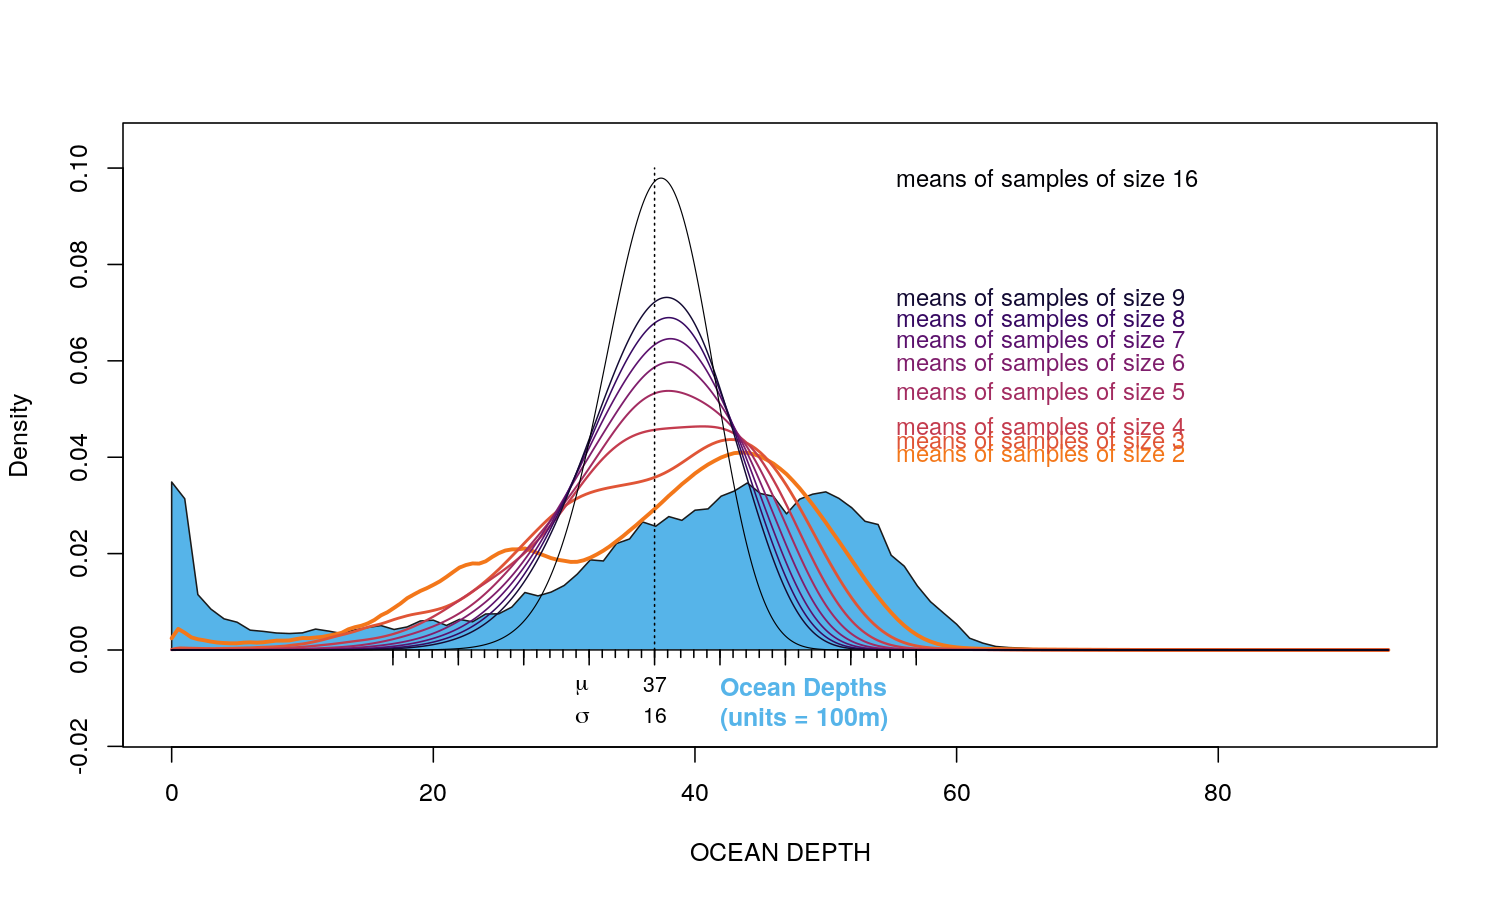
\includegraphics[width=\textwidth,height=0.8\textheight,keepaspectratio]{oceanAll.png}
%\includegraphics<3>{C}
\end{frame}



\begin{frame}[fragile]{Quadruple the work, half the benefit}

\framedgraphiccaption{ROOToceanAll.png}{When the sample size increases from 4 to 16, the spread of the sampling distribution for the mean is reduced by a half, i.e., the range is cut in half. This is known as the curse of the $\sqrt{n}$}
\end{frame}


\section{Confidence Intervals}


\begin{frame}{Key takeaways and next steps}
\begin{enumerate}
	\setlength\itemsep{2em}
	\item We've been exclusively talking about point estimates \pause
	\item How confident are we about these point estimates? \pause
	\item \textcolor{blue}{Thought experiment}: Estimate the average temperature in Montreal in August over the past 100 years. \pause  
	\item We're going into stat territory now. 
\end{enumerate}
\end{frame}


\begin{frame}{Confidence Interval}

\begin{defm}[Confidence Interval]
A level $C$ confidence interval for a parameter has two parts:
\begin{enumerate}
	\item An interval calculated from the data, \underline{usually} of the form $$\textrm{estimate} \pm \textrm{margin of error}$$ where the estimate is a sample statistic and the margin of error represents the accuracy of our guess for the parameter.
 \item A confidence level $C$, which gives the probability that the interval will capture the true parameter value in \textit{different possible samples}. That is, the confidence level is the success rate for the method
\end{enumerate}
\end{defm}

%\framedgraphic{6899rule.png}

\end{frame}

\frame{\frametitle{Confidence Interval: A simulation study}
	
	\vspace*{-0.1in}
	
	\begin{figure}
		\begin{center}
			\epsfig{figure=Part3Figs/CIplots.eps,width=3.2in,height=2.7in}
			\caption{\small{True parameter value is 2 (red line). Each horizontal black line represents a 95\% CI from a sample and contains the true parameter value. The blue CIs do not contain the true parameter value. 95\% of all samples give an interval that contains the population parameter.}}
		\end{center}
	\end{figure}
}





\begin{frame}{Confidence Intervals: we only get one shot}
\begin{itemize}
	\setlength\itemsep{2em}
	\item In practice, we don't take many simple random samples (``repeated'' samples) to estimate the population parameter $\theta$. \pause 
	\item Because the method has a 95\% success rate, all we need is one simple random sample to compute one CI. 
\end{itemize}
\end{frame}

\begin{frame}{Interpreting a frequentist confidence interval}
\begin{itemize}
			\setlength\itemsep{1em}
	\item The confidence level is the success rate of the method that produces the interval. \pause
	\item We don't know whether the 95\% confidence interval from a \underline{particular
	sample} is one of the 95\% that capture $\theta$ (the unknown population parameter), or one of the unlucky 5\% that miss. \pause
	\item To say that we are 95\% confident that the unknown value of $\theta$
	lies between $U$ and $L$ is shorthand for ``We got these numbers using a
	method that gives correct results 95\% of the time.''
\end{itemize}
\end{frame}

%\frame{\frametitle{Inference for a single population mean} So to
%perform inference, we want an estimator that is unbiased for the
%parameter of interest and that has a relatively small spread (low
%variability or high efficiency). \\ \ \\
%Examples - estimating the population mean $\mu$:
%\begin{itemize}
%\item What is the bias (if any) of $\frac{1}{n}\sum^n_{i=1}(x_i + 1)$?
%\item[] \item What is the bias (if any) of $\frac{1}{n}\sum^n_{i=1}x_i + \frac{1}{n}$?
%\item[] \item Which of the two estimators above would you prefer?
%\end{itemize}
%}


\begin{frame}{More about a frequentist confidence interval}

\begin{itemize}
	\item The confidence level of 95\% has to say something about the sampling procedure: \pause
		
	\begin{itemize}
		\item The confidence interval depends on the sample. If the sample had come out differently, the confidence interval would have been different. \pause
		\item With some samples, the interval 'estimate $\pm$ margin of error' does trap the population parameter (the word statisticians use is cover). But with other samples, the interval fails to cover.
	\end{itemize}
\pause
\item It's like buying a used car. Sometimes you get a lemon – a confidence interval which doesn't cover the parameter.

\framedgraphiccaption{lemon.jpg}{3 confidence intervals 'chasing' (taking a shot at) the population parameter $P$}
\end{itemize}
\end{frame}


\begin{frame}{More about a frequentist confidence interval}
\begin{itemize}
				\setlength\itemsep{2em}
	\item In the frequentist approach, $\theta$ is regarded as a fixed (but unknowable) constant, such as the exact speed of light to an infinite number of digits, or the exact mean depth of the ocean at a given point in time. \pause
	
	\item It doesn't ``fall'' or ``vary around'' any particular values; in contrast you can think of the statistic $\hat{\theta}$ ``falling'' or ``varying around'' the fixed (but unknowable) value of $\theta$
\end{itemize}
\end{frame}


\begin{frame}{Polling companies}
\begin{itemize}
					\setlength\itemsep{2em}
	\item Polling companies who say ``polls of this size are accurate to within so many percentage points 19 times out of 20'' are being statistically correct $\to$ they emphasize the \textbf{procedure} rather than what has happened in this specific instance. \pause 
	\item Polling companies (or reporters) who say ``this poll is accurate .. 19
	times out of 20'' are talking statistical nonsense -- this specific poll is either right or wrong. On average 19 polls out of 20 are ``correct''. But this
	poll cannot be right on average 19 times out of 20.
\end{itemize}
\end{frame}

\frame{\frametitle{Example: Inference for a single population mean} We begin
	with the (unrealistic) assumption that the population variance is
	known.
	\begin{itemize}
		\item Then the true variance of the sample mean is known!
		\item We can use \texttt{mosaic::xpnorm(q = c(-1.96, 1.96))} to find that there is a 95\% chance that a $\mathcal{N}$(0,1) random variable lies within 1.96 
		standard errors of the population mean of the distribution. So then:
		\[ P\left(-1.96 \le \frac{\bar{y}-\mu}{\sigma/\sqrt{n}} \le
		1.96\right) = 0.95 \]
		\item[]
	\end{itemize}
	What does allow us to learn about $\mu$? }

\frame{\frametitle{Example: Inference for a single population mean} We can
	use this probability statement about the standardized version of
	$\bar{y}$ to place bounds on where we think the true mean lies
	by examining the probability that $\bar{y}$ is within
	1.96$\frac{\sigma}{\sqrt{n}}$ of $\mu$. \\ \ \\
	
	$P\left(-1.96 \le \frac{\bar{y}-\mu}{\sigma/\sqrt{n}} \le
	1.96\right)$\\
	\[\begin{array}{ccl} \qquad & = & P\left(-1.96\frac{\sigma}{\sqrt{n}}
	\le \bar{y}-\mu \le +1.96\frac{\sigma}{\sqrt{n}}\right)\\
	\pause
	& = & P\left(-\bar{y}-1.96\frac{\sigma}{\sqrt{n}} \le
	-\mu \le -\bar{y}+1.96\frac{\sigma}{\sqrt{n}}\right)\\ \pause
	& = & P\left(\bar{y}+1.96\frac{\sigma}{\sqrt{n}} \ge
	\mu \ge \bar{y}-1.96\frac{\sigma}{\sqrt{n}}\right)\\ \pause
	& = & P\left(\bar{y}-1.96\frac{\sigma}{\sqrt{n}} \le \mu
	\le \bar{y}+1.96\frac{\sigma}{\sqrt{n}}\right)\\
	& = & 0.95\\
	& & \\
	\end{array}\]
	
	We call the interval
	$\left(\bar{y}-1.96\frac{\sigma}{\sqrt{n}},
	\bar{y}+1.96\frac{\sigma}{\sqrt{n}}\right)$ a \textbf{95\%
		confidence interval} for $\mu$. }

\frame{\frametitle{Example: Inference for a single population mean} So what does the CI allow us
	to learn about $\mu$?? \pause

	\begin{itemize}
							\setlength\itemsep{.5em}
		\item In classical (frequentist) statistics, we assume that the population
		mean, $\mu$ is a \textbf{fixed} but unknown value.
		\item With this view, it doesn't make sense to think of $\mu$ as
		having a distribution. Therefore we can't make probability statements about $\mu$. \pause
	\item What about the CI? It is made up of the sample mean
		and other fixed numbers (1.96, the square root of the known sample
		size $n$, and the known standard deviation, $\sigma$).
		\item \textcolor{blue}{\textbf{The CI is a random quantity.}}
		\item Remember: a random quantity is one in which the outcome is not
		known ahead of time. We don't know the lower and upper limits of the
		CI before the sample has been collected since we don't yet know the
		value of the random quantity $\bar{x}$.
	\end{itemize}
	
}

\frame{\frametitle{Example: Inference for a single population mean} So what
	does the CI allow us to learn about $\mu$??
	\begin{itemize}
							\setlength\itemsep{2em}
		\item It tells us that if we repeated this procedure again and again
		(collecting a sample mean, and constructing a 95\% CI), 95\% of the
		time, the CI would \textit{cover} $\mu$. \pause 
		\item That is, with 95\% probability, the \textit{procedure}
		will include the true value of $\mu$. Note that we are making \underline{a probability statement about the CI}, not about the parameter. \pause
		\item Unfortunately, \textcolor{blue}{we do not know whether the true value of $\mu$ is
			contained in the CI in the particular experiment that we have
			performed.}
	\end{itemize}
}


\begin{frame}{Interactive visualization of CIs}
\Large\href{http://rpsychologist.com/d3/CI/}{http://rpsychologist.com/d3/CI/}
\end{frame}



\begin{frame}[fragile]{Exercise: How deep is the ocean?}
%\begin{exm}[Confidence intervals in many samples]
\begin{enumerate}
	\item For your samples of $n=5$ and $n=20$ of depths of the ocean, calculate the
	\begin{enumerate}
		\item sample mean ($\bar{y}$)
		\item standard error of the sample mean ($SE_{\bar{y}}$)
	\end{enumerate}
	\item Calculate the 68\%, 95\% and 99\% confidence intervals (CI) for both samples of $n=5$ and $n=20$.
	\item Enter your results in the \href{https://docs.google.com/spreadsheets/d/1Mnxeq9nQcTdQycZ7S_62fYFiNC5_a3fibsyodzfwO58/edit?usp=sharing}{Google sheet} 
	\item Plot the CIs for each student using the following code:
	
\begin{knitrout}\scriptsize
\definecolor{shadecolor}{rgb}{0.969, 0.969, 0.969}\color{fgcolor}
\begin{alltt}
\hlkwd{plot}\hlstd{(dt}\hlopt{$}\hlstd{Mean.5.depths,} \hlnum{1}\hlopt{:}\hlkwd{nrow}\hlstd{(dt),} \hlkwc{pch}\hlstd{=}\hlnum{20}\hlstd{,}
\hlkwc{xlim}\hlstd{=}\hlkwd{range}\hlstd{(}\hlkwd{pretty}\hlstd{(}\hlkwd{c}\hlstd{(dt}\hlopt{$}\hlstd{lower.mean.5.66, dt}\hlopt{$}\hlstd{upper.mean.5.66))),}
\hlkwc{xlab}\hlstd{=}\hlstr{'Depth of ocean (m)'}\hlstd{,} \hlkwc{ylab}\hlstd{=}\hlstr{'Student (sample)'}\hlstd{,}
\hlkwc{las}\hlstd{=}\hlnum{1}\hlstd{,} \hlkwc{cex.axis}\hlstd{=}\hlnum{0.8}\hlstd{,} \hlkwc{cex}\hlstd{=}\hlnum{1.5}\hlstd{)}
\hlkwd{abline}\hlstd{(}\hlkwc{v} \hlstd{=} \hlnum{3700}\hlstd{,} \hlkwc{lty} \hlstd{=} \hlnum{2}\hlstd{,} \hlkwc{col} \hlstd{=} \hlstr{"red"}\hlstd{,} \hlkwc{lwd} \hlstd{=} \hlnum{2}\hlstd{)}
\hlkwd{segments}\hlstd{(}\hlkwc{x0} \hlstd{= dt}\hlopt{$}\hlstd{lower.mean.5.66,} \hlkwc{x1}\hlstd{=dt}\hlopt{$}\hlstd{upper.mean.5.66,}
\hlkwc{y0} \hlstd{=} \hlnum{1}\hlopt{:}\hlkwd{nrow}\hlstd{(dt),} \hlkwc{lend}\hlstd{=}\hlnum{1}\hlstd{)}
\end{alltt}

\end{knitrout}
	
\end{enumerate}
%\end{exm}
\end{frame}

\end{document}

\subsection{Confidence intervals: one sample}
\frame{\frametitle{Confidence intervals} Confidence intervals
	will appear again and again in statistics. They are of the
	general form
	\[\hbox{estimate} \pm \hbox{margin of error}.\]
	The estimate (and typically the margin of error as well) are
	computed from the sample data. \\ \ \\
	
	The confidence level chosen affects the width of the confidence
	interval through the size of the margin of error, and corresponds to
	the probability that the interval covers (includes) the true value
	of the parameter. }

\frame{\frametitle{CIs for a population mean when variance is known}
	How to construct a CI for the population mean?
	\begin{itemize}
		\item The CLT gives us that $\bar{y} \sim
		\mathcal{N}(\mu,\sigma/\sqrt{n})$ is approximately true when $n$ is
		large.
		\item We can standardize, to get $Z = \frac{\bar{y}-\mu}{\sigma/\sqrt{n}} \sim
		\mathcal{N}(0,1)$. \pause
		\item To find a CI with confidence level $\mathcal{C} = 1-\alpha$, we must look up
		the value $z^*$ on the $Z$-table such that $P(-z^* < Z < z^*) =
		1-\alpha$.
		\begin{itemize}
			\item That is, we want the value $z^*$ on the $Z$-table that gives a
			\textit{lower tail probability} of $\alpha/2$.
			\item Often this value is denoted $z^* = z_{\alpha/2}$; thus we have \[P(Z <
			-z_{\alpha/2}|Z\sim\mathcal{N}(0,1)) = \alpha/2,\] and \[P(Z >
			z_{\alpha/2}|Z\sim\mathcal{N}(0,1)) = \alpha/2.\]
		\end{itemize}
	\end{itemize}
} \frame{\frametitle{CIs for $\mu$ when $\sigma^2$ is known} Then we
	have:
	\[\begin{array}{ccl} 1-\alpha & = & P(-z_{\alpha/2} < Z < z_{\alpha/2})\\
	& & \\ & = & P\left(-z_{\alpha/2} < \frac{\bar{y}-\mu}{\sigma/\sqrt{n}} < z_{\alpha/2}\right)\\
	& & \\ & = & P\left(-z_{\alpha/2} <
	\frac{\mu-\bar{y}}{\sigma/\sqrt{n}} <
	z_{\alpha/2}\right)\\ \pause
	& & \\ & = & P\left(-z_{\alpha/2}\frac{\sigma}{\sqrt{n}} <
	\mu-\bar{y} <
	z_{\alpha/2}\frac{\sigma}{\sqrt{n}}\right)\\ \pause
	& & \\ & = & P\left(\bar{y}-z_{\alpha/2}\frac{\sigma}{\sqrt{n}}
	< \mu < \bar{y}+z_{\alpha/2}\frac{\sigma}{\sqrt{n}}\right)\\ & & \\
	\end{array}\]
	
	So a $(1-\alpha)$100\% CI for $\mu$ is
	\textcolor{blue}{$\bar{y}\pm
		z_{\alpha/2}\frac{\sigma}{\sqrt{n}}$.} }

%\frame{\frametitle{CIs for $\mu$ when $\sigma^2$ is known}
%Confidence intervals appear frequently in statistics, as we
%mentioned earlier, and they are often of the form
%\[\hbox{estimate} \pm \hbox{margin of error}.\]
%We can make this statement more precise, and say that typically, CIs
%are of the form \[\hbox{estimate} \pm
%z_{\alpha/2}\hbox{SE}_{\hbox{estimate}}.\] }

\frame{\frametitle{Interpreting confidence intervals} You have just
	computed a CI. There are 5 different conclusions that may be drawn:
	\begin{enumerate}
		\item The CI includes $\mu_0$, and neither end of the CI suggests
		anything clinically that might be interesting to me. I can conclude
		that this variable does not have any effect big enough to interest
		me.
		\begin{figure}
			\begin{center}
				\epsfig{figure=Part3Figs/CIfig1.eps,width=3.2in,height=2.5in}
			\end{center}
		\end{figure}
\end{enumerate} }
\frame{\frametitle{Interpreting confidence intervals} You have just
	computed a CI. There are 5 different conclusions that may be drawn:
	\begin{enumerate}
		\item[2.] The CI includes $\mu_0$, and one or both of the CI limits interests me
		clinically. The study suggests the variable might be important, but
		further study is needed.\\
		\begin{figure}
			\begin{center}
				\epsfig{figure=Part3Figs/CIfig2.eps,width=3.2in,height=2.5in}
			\end{center}
		\end{figure}
\end{enumerate} }
\frame{\frametitle{Interpreting confidence intervals} You have just
	computed a CI. There are 5 different conclusions that may be drawn:
	\begin{enumerate}
		\item[3.] The CI does not include $\mu_0$, and but both limits of the CI are too
		near zero to interest me clinically. Conclude that this variable
		does not have any effect big enough to interest me.
		\begin{figure}
			\begin{center}
				\epsfig{figure=Part3Figs/CIfig3.eps,width=3.2in,height=2.5in}
			\end{center}
		\end{figure}
\end{enumerate} }
\frame{\frametitle{Interpreting confidence intervals} You have just
	computed a CI. There are 5 different conclusions that may be drawn:
	\begin{enumerate}
		\item[4.] The CI does not include $\mu_0$, and some of the values inside the
		limits interest me clinically. The study suggests the variable may
		be important to me, but further study is needed. \begin{figure}
			\begin{center}
				\epsfig{figure=Part3Figs/CIfig4.eps,width=3.2in,height=2.5in}
			\end{center}
		\end{figure}
\end{enumerate} }
\frame{\frametitle{Interpreting confidence intervals} You have just
	computed a CI. There are 5 different conclusions that may be drawn:
	\begin{enumerate}
		\item[5.] The CI does not include $\mu_0$, and all of the values inside the
		limits interest me clinically. Conclude that this variable is
		important.\\
		\begin{figure}
			\begin{center}
				\epsfig{figure=Part3Figs/CIfig5.eps,width=3.2in,height=2.5in}
			\end{center}
		\end{figure}
\end{enumerate} }


\frame{\frametitle{Confidence intervals} Properties of confidence
	intervals:
	\begin{itemize}
		\item Decreasing the confidence level, $1-\alpha$, decreases the width of
		the CI. \pause
		\item Increasing the significance level, $\alpha$, decreases the width of
		the CI. \pause
		\item Increasing $n$ decreases the width of the CI.
		\begin{itemize}
			\item To halve the width of the CI, $n$ must be increased by a
			factor of 4.
		\end{itemize} \pause
		\item Decreasing the population variance, $\sigma^2$, decreases the width of
		the CI.
		\begin{itemize}
			\item This cannot always be accomplished.
			\item Improving measuring instruments (to reduce measurement error)
			can help.
			\item Changing the question to focus on a particular sub-population may
			also reduce the heterogeneity in the population.
		\end{itemize}
\end{itemize} }

\frame{\frametitle{CIs and sample size} Many plastics leach chemical
	compounds, which could have adverse effects in humans. Suppose very
	little is known about a particular compound, chemical P, although it
	is believed that concentrations of P greater than 1 unit/mL blood
	may be harmful. We wish to do a preliminary study to estimate the
	level of P concentrations in the bloodstream of Montrealers.
	
	\begin{itemize}
		\item Suppose a study of 100 people yields a CI of 0.05-6.03
		units/mL. \pause
		\item Is this study useful? \pause
		\item Is the study ethical? \pause
		\item Roughly how big would the study need to be to decrease the
		width of the CI to 0.6 units? \pause
	\end{itemize}
	How can we take advantage of what we know to have useful estimates?
	We need to determine what sample size is ``big enough.'' }

\frame{\frametitle{CIs and sample size} Note that the length of a CI
	is \[2\times\hbox{margin of error}.\]
	
	If we know $\sigma^2$ and we wish to obtain a CI of length, say,
	$2m$, we need only solve the equation
	\begin{eqnarray*}
		2m & = & 2\times\hbox{margin of error}\\
		& = & 2\times z_{\alpha/2}\sigma/\sqrt{n}
	\end{eqnarray*}
	which gives
	\[n = \qquad \qquad \]
	% \[n = \frac{z_{\alpha/2}\sigma}{m})^2 \]
}

\frame{\frametitle{Notes}
	\begin{itemize}
		\item The methods we have discussed are valid for data collected via a
		simple random sample from the population.
		\begin{itemize}
			\item Sample members must have been independently selected from the
			population.
			\item Other statistical methods exist for when a more complex (but still
			random) sampling scheme is used; these will not be taught in this
			course.
			\item If data were collected without care in a way that could
			produce bias (recall the example of determining the proportion of
			women at McGill), statistical methods cannot fix the study. \item[]
		\end{itemize} \pause
		\item The method we just examined requires us to know the value of
		$\sigma^2$. We study methods for when $\sigma^2$ is unknown
		shortly.\end{itemize} }

\frame{\frametitle{Notes}
	\begin{itemize}
		\item The margin of error used only guards against the
		variability (``error'') due to the chance variation in the sampling
		procedure.
		\item This does not guard against bias due to drop-out,
		non-compliance, non-random measurement error (e.g., self-reported
		weight), etc.
	\end{itemize}
}

\frame{\frametitle{Cautions}
	\begin{itemize}
		\item The sample mean is very sensitive to outlying data points.
		If data are not symmetric, transformations of the data or other more robust methods may
		be better alternatives. \pause
		\item[] \item If $n$ is small or the data are highly asymmetric, using the Normal
		distribution for the sample mean's distribution may not be a good
		approximation.
		\begin{itemize}
			\item We will discuss other methods that do not rely on this
			assumption later in the course (Part 5). \item[]
		\end{itemize} \pause
		\item Recall that the CI makes a probability statement about the
		\textit{procedure}, but \textcolor{blue}{cannot tell us whether the
			interval actually computed contains the true value of the
			parameter}.
	\end{itemize}
}




\end{document}



\begin{frame}[fragile]{Collecting data takes effort}

\begin{comment}

\Wider[9em]{
	\begin{figure}
		\begin{minipage}[h]{0.49\linewidth}
			\centering
			\includegraphics[scale=0.4]{cart_pruned-crop.pdf}
			\caption{Regression}
			\label{fig:a}
		\end{minipage}
		%\hspace{0.5cm}
		\begin{minipage}[h]{0.49\linewidth}
			\centering
			\includegraphics[scale=0.20]{class_tree-crop.pdf}
			\caption{Classification}
			\label{fig:b}
		\end{minipage}
	\end{figure}
}
\end{comment}


\begin{itemize}
	\item Today's class $\to$ regression
\end{itemize}

\end{frame}







\begin{frame}{How does CART work?}
	
	Roughly speaking, there are two steps~\cite{james2013introduction}:
	\pause 
	
	\begin{enumerate}
		\setlength\itemsep{1em}
		%\item Un arbre de régression et de classification se construit de manière itérative, en découpant à chaque étape la population en deux sousensembles\nocite{lopez2015arbres}
		%\item Le découpage s’effectue suivant des règles simples portant sur les variables	explicatives, en déterminant la règle optimalequi permet de construire deux populations les	plus différenciées en termes de valeurs de la variable à expliquer
		\item We divide the predictor space - that is, the set of possible values for
		$X_1, X_2,\ldots, X_p$, into $J$ non-overlapping and exhaustive regions,
		$R_1, R_2,\ldots, R_J$.
		\item For every observation that falls into the region $R_j$, we make the same
		prediction, which is simply the mean of the response values for the
		training observations in $R_j$.
	\end{enumerate}
\end{frame}







\begin{frame}{And if we continue...}

gdsgs

%\framedgraphic{area5.pdf}

\end{frame}

\begin{frame}{Stop if the number of observations is less than 20}

gsd

%\Wider[4em]{
%\includegraphics[scale=0.45]{tree5.pdf}
%}

\end{frame}


\section{The Details}


\begin{frame}{The Details}
	
The CART algorithm requires 3 components:

\begin{enumerate}
		  \setlength\itemsep{1.5em}
	\item Defining a criterion to select the best partition among all predictors.
	\item A rule to decide when a node is terminal, i.e., it becomes a leaf.
	\item Pruning the tree to avoid over-fitting.
\end{enumerate}

\end{frame}


\begin{frame}{1. Selecting the Best Partition}
	The objective is the find the regions $R_1, \ldots, R_J$ that minimize the squared error loss:
		
	\begin{equation}
		\sum_{j=1}^{J} \sum_{i \in R_j}(y_i - \hat{y}_{R_j})^2 \label{eq:obj1}
	\end{equation}
	
	\begin{itemize}
		\setlength\itemsep{1.5em}
		\item $\hat{y}_{R_j}$: the mean response for the training observations within the
		$j$th box \pause
		\item Finding the solution to~\eqref{eq:obj1} is computationally infeasible (\textit{NP-hard}). Why? 
	\end{itemize}
	
	
\end{frame}




\section{Comparison with a Linear Model}

\begin{frame}{Comparison: Linear Model vs. CART}
\vspace*{-0.25cm}

\ctable[pos=h!,doinside=\footnotesize]{lcc}{\tnote{\cmark: yes, \xmark: no}
}{
\FL
\textbf{Characteristic\tmark} & \textbf{\texttt{Linear Model}}   & \textbf{\texttt{CART}} \ML
\rowcolor{whitesmoke}
Linearity Assumption & \cmark &    \xmark    \\
& &  \\
Distributional Assumptions & \cmark & \xmark \\
& &  \\
\rowcolor{whitesmoke}
Robust to multicollinearity &  \xmark  &  \cmark   \\ 
%& &  \\
%High-dimensional data ($n << p$) & \xmark   & \cmark     \\
& &  \\
\rowcolor{whitesmoke}
Handles complex interactions &  \xmark  &  \cmark    \\
& &  \\
%Valeurs aberrantes  &    &      \\
\rowcolor{whitesmoke} 
Allows for missing data  & \xmark   &  \cmark    \\
& &  \\
Confidence Intervals, $p$-values & \cmark & \xmark \LL
}
\end{frame}




\begin{frame}[fragile]{Linear Model}
\begin{knitrout}\scriptsize
\definecolor{shadecolor}{rgb}{0.969, 0.969, 0.969}\color{fgcolor}
\begin{alltt}
\hlkwd{lm}\hlstd{(Salary} \hlopt{~} \hlstd{Years} \hlopt{*} \hlstd{Hits,} \hlkwc{data} \hlstd{= Hitters)}
\end{alltt}

\end{knitrout}


\end{frame}





\begin{frame}[allowframebreaks]
%\nocite{breiman1984classification}
	\nocite{friedman2001elements}
	\nocite{james2013introduction}
	\nocite{lopez2015arbres}
	\frametitle{References}
\printbibliography
\end{frame}


\begin{frame}[fragile]{Session Info}
	\tiny
	
\begin{knitrout}\tiny
\definecolor{shadecolor}{rgb}{0.969, 0.969, 0.969}\color{fgcolor}
\begin{verbatim}
R version 3.5.1 (2018-07-02)
Platform: x86_64-pc-linux-gnu (64-bit)
Running under: Ubuntu 18.04 LTS

Matrix products: default
BLAS: /usr/lib/x86_64-linux-gnu/openblas/libblas.so.3
LAPACK: /usr/lib/x86_64-linux-gnu/libopenblasp-r0.2.20.so

attached base packages:
[1] stats     graphics  grDevices utils     datasets  methods   base     

other attached packages:
 [1] tidyr_0.8.1        mosaic_1.4.0       Matrix_1.2-14     
 [4] mosaicData_0.17.0  ggformula_0.9.0    ggstance_0.3.1    
 [7] ggplot2_3.0.0.9000 lattice_0.20-35    dplyr_0.7.6       
[10] bindrcpp_0.2.2     knitr_1.20        

loaded via a namespace (and not attached):
 [1] Rcpp_0.12.18     pillar_1.3.0     compiler_3.5.1   highr_0.7       
 [5] plyr_1.8.4       bindr_0.1.1      tools_3.5.1      digest_0.6.16   
 [9] nlme_3.1-137     evaluate_0.11    tibble_1.4.2     gtable_0.2.0    
[13] pkgconfig_2.0.2  rlang_0.2.2      ggrepel_0.8.0    ggdendro_0.1-20 
[17] gridExtra_2.3    withr_2.1.2      stringr_1.3.1    grid_3.5.1      
[21] tidyselect_0.2.4 mosaicCore_0.6.0 glue_1.3.0       R6_2.2.2        
[25] pacman_0.4.6     purrr_0.2.5      magrittr_1.5     codetools_0.2-15
[29] backports_1.1.2  splines_3.5.1    scales_1.0.0     MASS_7.3-50     
[33] assertthat_0.2.0 colorspace_1.4-0 stringi_1.2.4    lazyeval_0.2.1  
[37] munsell_0.5.0    broom_0.5.0      crayon_1.3.4    
\end{verbatim}

\end{knitrout}

\end{frame}

\end{document}
